\documentclass[UTF8, a4paper, 12pt]{ctexart} % 将 15pt 替换为 12pt

% 设置页面边距
\usepackage[a4paper, margin=1.5cm]{geometry}

% 插入图片
\usepackage{graphicx}

% 插入代码
\usepackage{listings}

% 表格支持
\usepackage{booktabs}

% 数学公式支持
\usepackage{amsmath, amssymb}

% 超链接
\usepackage[colorlinks, linkcolor=blue, anchorcolor=blue, citecolor=blue]{hyperref}

% 参考文献
\usepackage{cite}

% 设置行间距
\usepackage{setspace}
\setstretch{1.5}

% 页眉页脚
\usepackage{fancyhdr} % 确保加载 fancyhdr 包
\pagestyle{fancy}
\fancyhf{}
\fancyhead[L]{\leftmark}
\fancyfoot[C]{\thepage}
\setlength{\headheight}{12.64723pt} % 增加页眉高度
\addtolength{\topmargin}{-0.64723pt} % 调整 topmargin 以补偿页眉高度的增加

% 标题格式
\usepackage{titlesec}
\titleformat{\section}{\Large\bfseries}{\thesection}{1em}{}
\titleformat{\subsection}{\large\bfseries}{\thesubsection}{1em}{}

% 文档信息
\title{洞头黄岙二期围涂工程白马堤设计}
\author{柳泽辰}
\date{\today}
\newpage

\begin{document}

\maketitle
\newpage
\section*{\centering}
\begin{abstract}
  在此处撰写您的中文摘要内容。
\end{abstract}
\newpage

\section*{\centering }
\begin{abstract}
  在此处撰写您的英文摘要内容。
\end{abstract}
\newpage
% 
\tableofcontents
\newpage

\section{背景介绍}

% 引言部分,介绍研究背景、意义和研究目标。
\subsection{工程背景}
洞头黄岙二期围涂工程位于浙江省温州市洞头区一带,洞头区作为浙江省重要的海岛经济区和渔业资源区,面临着海洋环境的不断变化以及自然灾害(如台风、海浪、高潮等)的频繁影响。在这种背景下,进行围涂工程不仅能够为当地的农业、渔业等产业提供保障,同时也能够为当地的经济发展创造更多的空间。
\subsection{工程位置}
洞头区是一个海岛区,全县由103个岛屿组成,素称“百岛之县”,总面积为\textbf{892.3平方公里},其中陆地面积为\textbf{100.3平方公里}。

人均耕地面积仅为\textbf{0.12亩},人多地少的矛盾日益突出。围涂造地不仅可以发展农业、水产养殖业,更重要的是缓解洞头县人多地少、经济发展土地不足之间矛盾的重要途径。

洞头区黄岙二期围涂工程位于洞头区大门岛南部黄岙海涂面上,界于北纬27°57′33″$\sim$27°59′18″,东经121°03′00″$\sim$121°05′10″之间,系已围涂开发的黄岙一期工程的外围部分。

自20世纪70年代黄岙一期工程围涂后,外侧涂面已淤积较高,具备了较好的围涂条件。
\begin{figure}[h]
    \centering
    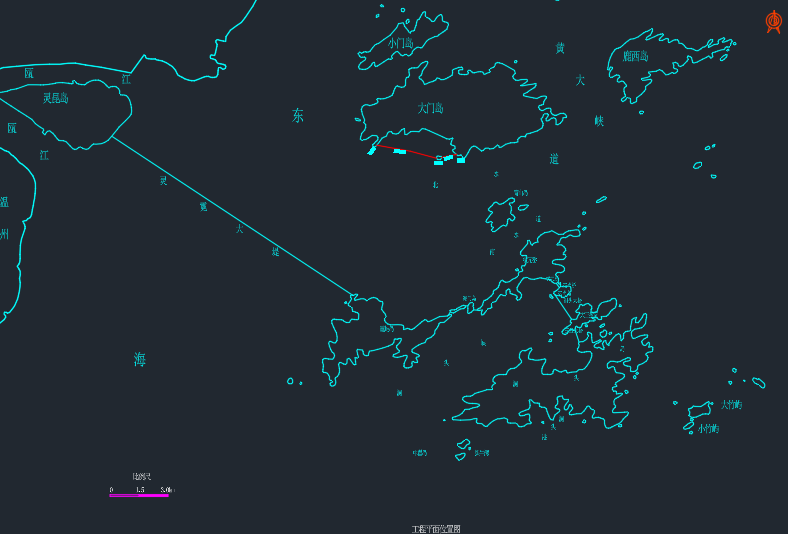
\includegraphics[width=0.7\textwidth]{9.png}
    \caption{洞头黄岙二期围涂工程位置图}
    \label{fig:location}
    
\end{figure}

\subsection{坐标高程系}
\textbf{本工程设计采用温州市独立坐标系,高程采用洞头本岛高程基准(零高程=吴凇基准高程-0.16m=1985国家高程基准+1.72m)。}

\begin{figure}[h]
    \centering
    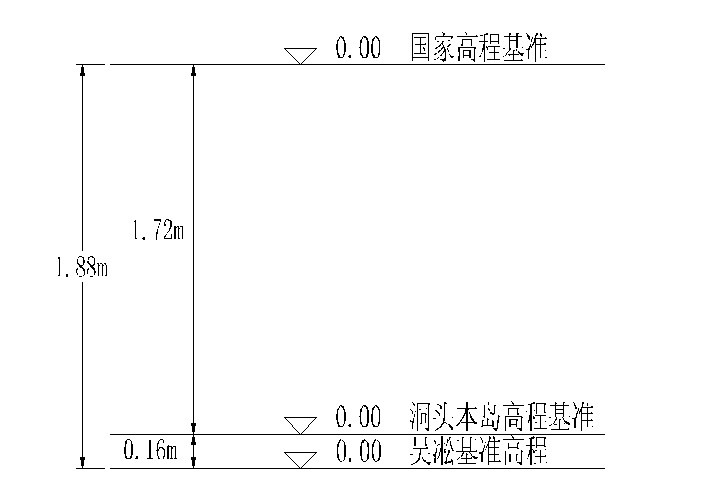
\includegraphics[width=0.7\textwidth]{1.png}
    \caption{各高程系相对位置示意图}
    \label{fig:location}
\end{figure}

\newpage
\subsection{工程意义}
白马堤作为黄岙二期围涂工程的重要组成部分,主要功能是防止海水倒灌、提高沿海区域的防洪能力、保护农业和渔业资源。
该堤坝的设计除了要保证其防洪防潮的功能外,还要充分考虑生态环境的保护,避免在围涂过程中对自然环境造成破坏。
\subsection{工程目标}
\subsubsection{经济发展目标}
\textbf{增加耕地资源}:该工程通过围涂的方式,将海域转化为可耕种的土地,增加耕地面积,为农民提供更多的种植土地。这对于促进当地农业发展、提高农民收入具有重要作用。
\par \textbf{推动产业升级}:该工程可能带动当地农业、渔业等传统产业向更高效、更可持续的方向发展。同时,也为相关基础设施建设(如交通、能源、灌溉等)提供了支持,促进区域经济的全面发展。
\par \textbf{支持城市化进程}:围涂后的土地可以用于开发住宅、商业、工业用地,为洞头及周边地区的城市化提供土地资源,支持地方经济的快速增长。

\subsubsection{生态环境改善与可持续发展}
\textbf{生态保护与恢复}
围涂工程要与生态保护紧密结合,避免对海洋环境造成过度破坏。通过对白马堤的开发,可以加强对海岸线的防护,减少海水侵蚀,同时通过科学规划恢复湿地、增加绿化。
\par \textbf{生态系统服务功能提升}
通过科学设计,围涂工程可以加强湿地的生态功能,促进生物多样性的保护,并为区域提供天然的生态服务,如水质净化、气候调节等。
\par \textbf{生态保护与恢复}
白马堤作为防护堤,可以有效防止海水倒灌、潮汐灾害、风暴潮等自然灾害,为当地人民的生产生活提供保障。
\subsubsection{社会发展目标}
\par \textbf{改善居民生活条件}
围涂工程的实施将为当地居民提供更多的耕地资源,改善他们的生活条件,提高生活水平。
\par \textbf{促进社会和谐发展}
围涂工程的实施将为当地居民提供更多的就业机会,促进社会的和谐发展。同时,通过对生态环境的保护与恢复,增强居民的环保意识,提高社会整体素质。
\par \textbf{提升区域形象}
随着围涂工程的推进,洞头的整体基础设施和区域环境得到改善,可以提升地区的吸引力,吸引更多投资与人才,从而推动地方社会的综合发展。

\subsection{参考规范}
% 添加有序列表
\begin{enumerate}
    
    \item 《港口与航道水文规范》(2022版)
    \item 《港口与航道水文规范》(JTS145—2015)
    \item  15~16. JTS 154—2018 防波堤与护岸设计规范
    \item  DB32T 2709-2014 水利工程概算编制规定
    \item  GB 50286-2013  堤防工程设计规范
    \item JTS 147-1-2010 港口工程地基规范
    \item GB 50288-2018 灌溉与排水工程设计标准 (1)
    \item JTS 147-2-2009 真空预压加固软土地基技术规程
    \item JTS 181-5-2012 疏浚与吹填工程设计规范
    \item SL 239-1999 堤防工程施工质量评定与验收规程(试行)
    \item SL 260-1998 堤防工程施工规范
    \item SL 265-2016 水闸设计规范
    \item 港口工程地基规范
    \item 港口工程荷载规范
    \item 浙江省海塘工程技术规定(上)
    \item 浙江省海塘工程技术规定(上)
    
    \end{enumerate}

\subsection{设计内容}

本次设计内容主要有:总平面布置;设计波浪要素的确定;对东围堤进行工程设计;
龙口水力计算;施工组织设计。

\subsection{工程等级}
温州市洞头县黄岙二期围涂工程保护对象为洞头区大门岛南部黄岙海涂面,防护人口规模 5
万余人,围涂面积 4260 亩,根据《浙江省海塘工程技术规定》,工程等级应为 IV 级。
不过洞头区为海岛区,工程等级应提高一个级别,定位 III 级海塘工程。其中,海堤、
水闸等主要建筑物级别定位 3 级,施工围堰等临时建筑物定位为 5 级。
\subsection{设计标准}
\begin{enumerate}
    \item 海堤水闸的挡潮防浪标准为:按 50 年一遇高潮位加 50 年一遇风浪爬高进行设计。其中,海堤允许部分越浪,水闸不允许越浪。
    \item 龙口度汛设计标准为汛期 20 年一遇高潮位及典型潮型。
    \item 堤口设计标准为非汛期 10 年一遇高潮位及典型潮型。
    \item 围堰堆项高程确定标准为非汛期 10 年一遇高潮位加安全超高。
    \item 排水闸按城市排涝标准的暴雨公式进行计算,并用 20 年一遇 24 小时暴雨和养殖排水叠加,外海为多年平均最高潮位工况进行校核,取其不利着确定排水闸规模。
\end{enumerate}

\section{施工条件}
% 综述相关领域的研究现状和已有工作。
\subsection{地形地貌}
洞头区,侵蚀丘陵地貌分布广泛,约占全区陆地面积的91\%。其中高丘陵(海拔250米以上)主要分布于大门岛以及鹿西、霓屿、状元岙等岛的中部和洞头岛的西部,山坡较陡,一般坡度$30^{\circ}\sim40^{\circ}$,特别是边缘地带,常有大于40°的陡坡或陡崖出现;顶部较平缓,坡度一般$15^{\circ}\sim25^{\circ}$。最高山峰烟墩山位于大门岛,海拔391.8米。高丘陵以凸形坡及直线形坡为主,部分地段为复合形坡。低丘陵(海拔低于250米)主要分布于洞头岛、半屏岛、三盘岛、小门岛以及鹿西、霓屿、状元岙等岛边角部位,山顶部较平缓,坡度为$10^{\circ}\sim25^{\circ}$,山坡坡度$25^{\circ}\sim35^{\circ}$,局部坡麓地带有超过35°陡坡及陡崖。低丘陵的山坡地形以凸形坡和直线形坡为主,局部为阶梯状复合形坡。
\par 堆积地貌主要分布于大门岛、灵昆岛和洞头岛,分布零星。其中洪积平原零星分布于大岛屿的沟谷及山麓地带,上游坡度$10^{\circ}\sim15^{\circ}$,下游坡度$3^{\circ}\sim10^{\circ}$。
\par 海积平原主要分布于洞头岛、灵昆岛、大门岛及小门岛,在霓屿岛及半屏岛亦有小块分布,地势平坦。境内无大河发育,溪流多发源于山体中部,向四周呈辐射状独流入海,其特点是数量多、流域面积小,长度短,比降大,枯水期多断流。

\subsection{地质条件}
\subsubsection{概述}
本章节是由浙江省围海建设股份有限公司2004年2月编制的《洞头县黄岙二期围涂工程地质勘察报告》摘编,工程地质平、剖面图见原工程地质勘察报告附图。勘察外业工作自2003年12月25日至2004年01月05日止,
共计完成取土孔24个,静力触探孔3个,十字板试验孔19个,完成的勘探工作量见下表1。
\begin{table}[h]
    \centering
    \caption{堤线勘探工作量统计表}
    \resizebox{\textwidth}{!}{ % 缩放表格以适应页面宽度
        \begin{tabular}{|c|c|c|c|c|c|}
            \hline
            位置 & 剖面长度(米) & 取土孔(米/个) & 静力触探孔(米/个) & 十字板孔(试验次数/个) & 原状土样(筒) \\ \hline
            推荐堤线 & 3900 & 679.4/19 & 200.0/5 & 256 & - \\ \hline
            比较堤线 & 3765 & 172.0/5 & 91.9/3 & 560.0/14 & 62 \\ \hline
        \end{tabular}
    }
    \label{tab:exploration_statistics}
\end{table}

\subsubsection{区域地质概况}
围区所在地属台州湾——沙埕港低山丘陵河口堆积平原区所属乐清湾低山丘陵海湾岛屿亚区。在地质构造上属华夏褶皱带,受北北东向构造及其配套的北西向和北东东向构造控制比较显著,在地貌上反映比较明显,如台州湾外至洞头诸岛,总体皆呈北北西方向展布。而单个岛屿则大多数作北东东方向延伸。地貌多呈丘陵地形,少数低山峰林等地形则多为熔结凝灰岩、流纹(斑)岩、石英正长岩等坚硬岩石构成。
区内的低山丘陵多由晚侏罗世火山——沉积岩及燕山期侵入岩构成,第四纪沉积地层皆为全新统滨海组海相淤积土层。
第四纪早期本区属上升阶段,中更新世后期转为下沉,全新世中期以后又回升,直至近期上升仍较显著。
第四纪地层多为全新统滨海组冲海相沉积土层,其上部为灰黄色粉土,局部为粉质粘土层,下部为灰黄$\sim$灰色的粉土、粉砂及细砂层。
根据《中国地震动参数区划图》(GB 18306-2001),工程区地震动峰值加速度为0.05g(地震基本烈度为Ⅵ度),地震动反应谱特征周期为0.65s(按Ⅰ区软弱场地划定)。
\subsubsection{堤基工程地质条件}
根据钻探揭露,围堤左右堤肩岩石皆为燕山晚期第三次侵入的中细粒钾长花岗岩,第四纪地层按土的工程地质特性可分为六个工程地质层及十六个亚层。
\subsubsection{堤基工程地质条件}
根据钻探揭露,围堤左右堤肩岩石皆为燕山晚期第三次侵入的中细粒钾长花岗岩,第四纪地层按土的工程地质特性可分为六个工程地质层及十六个亚层。

\par 1)1-1层淤泥($mQ4$)\\
滨海相沉积土,灰黄色,仅在ZS20孔中揭露,顶板出露涂面,厚1.3m,土质呈饱和、流塑状态。其主要的物理力学指标:
\[
w=55.9\%,\ \rho=1.70\, \text{g/cm}^3,\ \rho_d=1.09\, \text{g/cm}^3,\ E_s{_\perp}=1.548\, \text{MPa},\ C=4.6\, \text{kPa},\ \varphi=10^\circ,\ f_k=58\, \text{kPa}
\]

\par 2)1-2层淤泥质粉质粘土($mQ4$)\\
滨海相沉积土,灰黄色,仅在ZS24孔中揭露,顶板出露涂面,厚2.5m,土质呈饱和、流$\sim$软塑状态。其主要物理力学指标:
\[
w=36.6\%,\ \rho=1.85\, \text{g/cm}^3,\ \rho_d=1.35\, \text{g/cm}^3,\ E_s{_\perp}=3.266\, \text{MPa},\ C=12\, \text{kPa},\ \varphi=5^\circ,\ f_k=90\, \text{kPa}
\]

\par 3)1-3层含泥细砂($mQ4$)\\
灰$\sim$灰黄色,除ZS20与ZS24孔外,分布于全区,顶板出露涂面,厚0.0$\sim$5.2m,一般厚2.0$\sim$3.2m,土质不均匀但稍好,含泥量变化较大,固结排水条件较好,土质呈饱和、湿、稍松状态。其主要物理力学指标:
\[
w=39.9\%,\ \rho=1.80\, \text{g/cm}^3,\ \rho_d=1.27\, \text{g/cm}^3,\ E_s{_\perp}=5.318\, \text{MPa},\ C=6\, \text{kPa},\ \varphi=20^\circ,\ f_k=120\, \text{kPa}
\]

\par 4)1-4层淤泥夹砂($mQ4$)\\
海相淤积土,灰$\sim$灰黄色,分布于全区,顶板高程出露涂面$\sim$-12.0m,厚1.0$\sim$6.2m,含砂量不均匀,粉细砂多呈薄饼状分布,局部呈砂团状,固结排水条件稍好,呈饱和、流塑状态。其主要物理力学指标:
\[
w=51.7\%,\ \rho=1.71\, \text{g/cm}^3,\ \rho_d=1.13\, \text{g/cm}^3,\ E_s{_\perp}=2.317\, \text{MPa},\ C=3.5\, \text{kPa},\ \varphi=2.5^\circ,\ f_k=75\, \text{kPa}
\]

\par 5)2-1层淤泥($mQ4$)\\
海相淤积土,灰$\sim$青灰色,呈厚层状分布于全区,顶板高程-4.3$\sim$-12.8m,厚5.9$\sim$16.5m,土质稍均匀但较差,呈饱和、流塑状态。其主要物理力学指标:
\[
w=68.5\%,\ \rho=1.60\, \text{g/cm}^3,\ \rho_d=0.95\, \text{g/cm}^3,\ E_s{_\perp}=1.240\, \text{MPa},\ C=6.5\, \text{kPa},\ \varphi=1.6^\circ,\ f_k=50\, \text{kPa}
\]

\par 6)2-2层淤泥($mQ4$)\\
海相淤积土,与2-1基本为同一土层,仅埋深较之为深,土质相对较2-1层为好。灰色,呈厚层状分布于全区,顶板高程-14.3$\sim$-26.3m,厚3.0$\sim$22.2m,土质稍差,呈饱和、流$\sim$软塑状态。其主要物理力学指标:
\[
w=61.7\%,\ \rho=1.63\, \text{g/cm}^3,\ \rho_d=1.01\, \text{g/cm}^3,\ E_s{_\perp}=1.804\, \text{MPa},\ C=12.4\, \text{kPa},\ \varphi=2.8^\circ,\ f_k=65\, \text{kPa}
\]

\par 7)2-3层淤泥质粘土($mQ4$)\\
海相淤积土,灰色,局部缺失,顶板高程-22.7$\sim$-29.2m,厚0$\sim$8.0m,一般厚1.5$\sim$3.0m,土质较2-1、2-2为好,呈饱和、软塑状态。其主要物理力学指标:
\[
w=51.4\%,\ \rho=1.70\, \text{g/cm}^3,\ \rho_d=1.13\, \text{g/cm}^3,\ E_s{_\perp}=1.707\, \text{MPa},\ C=14.1\, \text{kPa},\ \varphi=4.1^\circ,\ f_k=70\, \text{kPa}
\]

\par 8)2-4层淤泥质粉质粘土($mQ4$)\\
灰色,呈透镜体分布,顶板高程-27.9$\sim$-33.1m,厚0$\sim$4.0m,一般厚2.5$\sim$3.0m,土质稍好,呈饱和、软塑状态。其主要物理力学指标:
\[
w=40.6\%,\ \rho=1.78\, \text{g/cm}^3,\ \rho_d=1.27\, \text{g/cm}^3,\ E_s{_\perp}=3.160\, \text{MPa},\ C=15.5\, \text{kPa},\ \varphi=8.6^\circ,\ f_k=90\, \text{kPa}
\]

\par 9)2-5层淤泥质粘土($mQ4$)\\
灰色,呈透镜体分布,顶板高程-28.7$\sim$-34.0m,厚0$\sim$8.5m,一般厚大于2.0m,土质稍好于2-3层,呈饱和、软塑状态。其主要物理力学指标:
\[
w=49.2\%,\ \rho=1.71\, \text{g/cm}^3,\ \rho_d=1.15\, \text{g/cm}^3,\ E_s{_\perp}=2.606\, \text{MPa},\ C=15.7\, \text{kPa},\ \varphi=5.4^\circ,\ f_k=80\, \text{kPa}
\]

\par 10)3层粘土($mQ4$)\\
灰色,在推荐堤线青菱屿——乌仙头中段出现,向两侧尖灭,顶板高程-25.5$\sim$-36.1m,厚0$\sim$6.0m,一般厚3.5m左右,土质稍好,呈饱和、软塑状态。其主要物理力学指标:
\[
w=49.5\%,\ \rho=1.70\, \text{g/cm}^3,\ \rho_d=1.14\, \text{g/cm}^3,\ E_s{_\perp}=2.756\, \text{MPa},\ C=15.4\, \text{kPa},\ \varphi=5.8^\circ,\ f_k=85\, \text{kPa}
\]

\par 11)4层淤泥质粘土($mQ4$)\\
灰色,在推荐堤线青菱屿——乌仙头中段出现,向两侧尖灭,顶板高程-30.8$\sim$-42.3m,未钻穿,揭露最大厚度5.5m,土质呈饱和、流塑状态。其主要物理力学指标:
\[
w=54.8\%,\ \rho=1.66\, \text{g/cm}^3,\ \rho_d=1.07\, \text{g/cm}^3,\ E_s{_\perp}=2.4102\, \text{MPa},\ C=13.4\, \text{kPa},\ \varphi=5.1^\circ,\ f_k=75\, \text{kPa}
\]

\par 12)5-1层粉质粘土($mQ4$)\\
灰色,仅在ZS2孔中揭露,顶板高程-40.3m,未钻穿,揭露最大厚度6.5m,土质稍好,呈饱和、软塑状态。其主要物理力学指标:
\[
w=38.5\%,\ \rho=1.78\, \text{g/cm}^3,\ \rho_d=1.30\, \text{g/cm}^3,\ E_s{_\perp}=2.978\, \text{MPa},\ C=16.0\, \text{kPa},\ \varphi=4.4^\circ,\ f_k=90\, \text{kPa}
\]

\par 13)5-2层粘土($mQ4$)\\
滨海相沉积土,灰色,在推荐堤线青菱屿——乌仙头中段出现,向两侧尖灭,顶板高程-37.0$\sim$-48.5m,未钻穿,揭露最大厚度4.0m,土质均匀,稍好,呈饱和、软$\sim$可塑状态。其主要物理力学指标:
\[
w=48.4\%,\ \rho=1.71\, \text{g/cm}^3,\ \rho_d=1.17\, \text{g/cm}^3,\ E_s{_\perp}=4.066\, \text{MPa},\ C=22.0\, \text{kPa},\ \varphi=5.0^\circ,\ f_k=100\, \text{kPa}
\]

\par 14)6-1层淤泥质粘土夹砾砂($al$-$mQ3$)\\
冲—海相淤积土,灰$\sim$灰褐色,分布于推荐堤线两侧,顶板高程-30.5$\sim$-32.1m,厚1.9$\sim$3.4m,土质不均但稍好,呈饱和、软塑、稍松状态。其主要物理力学指标:
\[
w=31.4\%,\ \rho=1.91\, \text{g/cm}^3,\ \rho_d=1.45\, \text{g/cm}^3,\ E_s{_\perp}=3.152\, \text{MPa},\ C=9.8\, \text{kPa},\ \varphi=20.8^\circ,\ f_k=95\, \text{kPa}
\]

\par 15)6-2层粘质粉土($al$-$mQ3$)\\
灰$\sim$灰褐色,仅在ZS19孔中揭露,顶板高程-34.1m,未钻穿,揭露最大厚度3.5m,土质稍好,呈饱和、湿、稍密状态。其主要物理力学指标:
\[
w=33.3\%,\ \rho=1.98\, \text{g/cm}^3,\ \rho_d=1.42\, \text{g/cm}^3,\ C=19.4\, \text{kPa},\ \varphi=23.1^\circ,\ f_k=125\, \text{kPa}
\]

\par 16)6-3层砾砂夹贝壳($al$-$mQ3$)\\
灰$\sim$灰黄色,仅在D—D'剖面中揭露,顶板高程-26.4$\sim$-35.5m,未钻穿,揭露最大厚度2.3m,富含贝壳,砂中石英颗粒较多,结构稍松。其主要物理力学指标:
\[
w=22.7\%,\ \rho=1.98\, \text{g/cm}^3,\ \rho_d=1.61\, \text{g/cm}^3,\ E_s{_\perp}=7.801\, \text{MPa},\ f_k=135\, \text{kPa}
\]

\subsubsection{建筑材料}
\par 1)石料:围区两堤肩皆为可采用的石料,储量丰富,质地也较好,山体岩性为中细粒钾长花岗岩,岩体较完整。
\par 2)砂料:本地位于瓯江口,砂源充足,可就近取用。
\par 3)土料:根据围涂需要,建议在堤线中段(B—B’剖面$\sim$青菱屿)堤线内、外200m以远取土,并浅挖为宜。


\subsection{水文气象}
\subsubsection{流域情况}
黄岙二期围涂工程位于浙江省温州市洞头县大门岛南部黄岙海涂上,围涂南侧临海,与灵霓海堤工程和霓屿岛相望,北侧靠大门岛陆域,东濒东海,西隔温州湾与乐清市相距9.5km。界于北纬27°52′33″$\sim$27°53′10″,东经121°07′13″$\sim$121°08′21″之间。

洞头县是全国12个海岛县之一,县域总面积892.3km\textsuperscript{2},其中陆地面积100.3km\textsuperscript{2},海域面积为792km\textsuperscript{2},海岛岸线总长331km。大门岛位于洞头列岛的东北部,陆域面积为28.7km\textsuperscript{2}。

黄岙二期围涂工程西起下乌仙的乌仙头嘴,东至潭头,东西向长约4.0km,南北向平均离岸1km 左右。涂面自北向南倾斜,基本上是北高南低,从北侧的2.0$\sim$2.2m 向南降到-2.5m左右,面积为3.73km\textsuperscript{2}。

围区和内陆黄岙一期平原地带被三面的山地和丘陵所包围。围区总流域面积为14.84km\textsuperscript{2},其中上游流域面积为11.11km\textsuperscript{2}(包括山地5.73km\textsuperscript{2}和黄岙一期2.68km\textsuperscript{2}),围区面积3.73km\textsuperscript{2}。黄岙二期围涂工程位置见附图。



\subsubsection{气象条件}
设计流域附近设有洞头气象站,站址位于洞头县洞头乡后坑村上后坑山顶,东经121°09′,北纬27°50′,观测场地面海拔68.6m。

洞头气象站资料均据中央气象局制定的《全国地面基本气候资料统计方法》及其补充规定进行整编,成果可靠,为本工程气象要素统计的主要依据。

据洞头气象站实测资料统计:
\begin{itemize}
    \item 多年平均气温为17.3℃,极端最高气温35.7℃,极端最低气温-4.1℃;
    \item 多年平均水汽压17.9hPa,多年平均相对湿度80\%,多年平均蒸发量1538.3mm(20cm蒸发皿观测值);
    \item 多年平均无霜期329天,多年平均日照时数1932.4小时;
    \item 多年平均风速5.3m/s,最大风速38.0m/s,相应风向为SSW。
\end{itemize}

洞头站地面气候特征值见表2。本工程地处我省东南部,濒临东海,属亚热带季风气候区,具有明显的海洋性气候特征。气候温和湿润,四季分明,雨量丰沛,日照充足,无霜期长。

多年平均雨日为156日(洞头站降水日数统计见表3)。设计流域附近的洞头站多年平均降水量为1220.5mm,其中最大年为1752.9mm(1962年),最小年为647.7mm(1971年)。

流域降水量不仅年际变化较大,而且年内分配不均:
\begin{itemize}
    \item 冬季受北方冷空气控制,低温少雨;
    \item 春季大陆冷高压衰退,副热带高压北进,冷暖气团交绥,形成绵绵春雨;
    \item 春末夏初,太平洋高压渐向大陆推进,造成连续降水,俗称梅雨季节;
    \item 7至10月间,受太平洋副热带高压控制,天气炎热,台风活动频繁。
\end{itemize}

台风是影响本地区的主要灾害性天气之一。在其活动过程中,伴随着狂风、暴雨、巨浪和风暴潮,往往给沿海地区的人民生命财产带来极大危害。
\begin{table}[h]
    \centering
    \caption{洞头气象站气象统计表}
    \resizebox{\textwidth}{!}{
    \begin{tabular}{|c|c|c|c|c|c|c|c|c|c|c|c|c|c|}
        \hline
        项目 & 一月 & 二月 & 三月 & 四月 & 五月 & 六月 & 七月 & 八月 & 九月 & 十月 & 十一月 & 十二月 & 全年 \\ \hline
        平均气温(℃) & 7.6 & 7.4 & 9.9 & 14.6 & 19.1 & 23.4 & 26.8 & 27.3 & 24.8 & 20.6 & 15.6 & 10.3 & 17.3 \\ \hline
        极端最高气温(℃) & 21.8 & 22.2 & 22.7 & 24.9 & 28.5 & 31.4 & 33.9 & 35.7 & 33.7 & 30.8 & 26.6 & 22.5 & 35.7 \\ \hline
        极端最低气温(℃) & -3.6 & -2.1 & 0.2 & 3.5 & 9.2 & 13.4 & 18.9 & 20.4 & 14.7 & 8.6 & 2.8 & -2.3 & -3.6 \\ \hline
        平均水汽压(hPa) & 7.9 & 8.3 & 10.2 & 14.5 & 19.7 & 26.2 & 31.1 & 30.8 & 25.2 & 18.6 & 13.1 & 9.0 & 17.9 \\ \hline
        平均相对湿度(\%) & 73 & 78 & 82 & 86 & 88 & 90 & 88 & 85 & 79 & 75 & 71 & 69 & 80 \\ \hline
        平均降水量(mm) & 49.7 & 75.5 & 119.4 & 151 & 182.3 & 168.6 & 85.6 & 139.9 & 137.4 & 73.3 & 70.3 & 41.8 & 1294.7 \\ \hline
        平均蒸发量(mm) & 84.8 & 68.7 & 82.0 & 94.9 & 107.8 & 126.0 & 189.2 & 198.3 & 175.9 & 171.9 & 132.4 & 106.6 & 1538.3 \\ \hline
        平均风速(m/s) & 5.9 & 5.8 & 5.1 & 4.0 & 4.2 & 5.0 & 5.6 & 5.2 & 5.5 & 6.1 & 6.2 & 5.6 & 5.3 \\ \hline
        最大风速(m/s) & 21.3 & 20.0 & 19.3 & 21.0 & 19.0 & 21.3 & 34.0 & 38.0 & 18.7 & 31.0 & 20.3 & 19.0 & 38.0 \\ \hline
        最大风速相应风向 & NNE & S & NNE & 2G & NE & SSW & NNW & SSW & NNE & S & NNE & 2G & SSW \\ \hline
   
    \end{tabular}
    }
    \label{tab:meteorological_statistics}
\end{table}

\begin{table}[h]
    \centering
    \caption{洞头气象站降水日数统计表}
    \resizebox{\textwidth}{!}{
    \begin{tabular}{|c|c|c|c|c|}
        \hline
        月份 & $\geq 0.1$mm降水日数(d) & $\geq 10$mm降水日数(d) & $\geq 25$mm降水日数(d) & $\geq 50$mm降水日数(d) \\ \hline
        1  & 12.1 & 1.4 & 0.1 & 0.0 \\ \hline
        2  & 15.1 & 2.6 & 0.2 & 0.0 \\ \hline
        3  & 17.9 & 4.1 & 0.9 & 0.1 \\ \hline
        4  & 17.9 & 5.5 & 1.6 & 0.2 \\ \hline
        5  & 18.8 & 5.9 & 2.1 & 0.5 \\ \hline
        6  & 16.1 & 5.1 & 2.2 & 0.6 \\ \hline
        7  & 9.5  & 1.9 & 0.9 & 0.5 \\ \hline
        8  & 12.3 & 3.3 & 1.4 & 0.7 \\ \hline
        9  & 12.1 & 3.5 & 1.5 & 0.7 \\ \hline
        10 & 8.5  & 2.4 & 1.0 & 0.2 \\ \hline
        11 & 8.6  & 2.2 & 0.8 & 0.2 \\ \hline
        12 & 7.3  & 1.2 & 0.3 & 0.1 \\ \hline
        全年 & 156  & 39  & 13  & 4   \\ \hline
    \end{tabular}
    }
    \label{tab:rainfall_days}
\end{table}
\subsubsection{水文基本资料}
设计流域内无水文测站。附近雨量站有洞头、龙湾、乐清、玉环等站,潮位站有洞头、龙湾、坎门等站。其中洞头站降水观测资料起始于1957年,1967年缺测,至今共有48年系列。洞头站潮位观测资料起始于1984年,至今共有22年系列。龙湾站降水观测资料起始于1960年,至今共有46年系列。龙湾潮位观测资料起始于1959年,至今共有47年系列。坎门站潮位观测资料起始于1958年,至今共有48年系列。我省沿海的小河站有施家桥等水文站,海岛水文站有舟山本岛上的长春岭水文站。
\begin{table}[h]
    \centering
    \caption{水文站点基本信息表}
    \begin{tabular}{|c|c|c|c|c|}
        \hline
        站名 & 设立年份 & 集水面积(km\textsuperscript{2}) & 观测项目 & 备注 \\ \hline
        洞头 & 1957 & - & 潮水位、降水量 & 潮水位观测始于1984年 \\ \hline
        龙湾 & 1959 & - & 潮水位、降水量 & - \\ \hline
        乐清 & 1951 & - & 降水量 & - \\ \hline
        玉环 & 1933 & - & 降水量 & 连续系列始于1952年 \\ \hline
        坎门 & 1958 & - & 潮水位、降水量 & - \\ \hline
        施家桥 & 1956 & 41.6 & 降水量、水位、流量等 & 1961-1962年缺测 \\ \hline
        长春岭 & 1980 & 3.8 & 降水量、水位、流量等 & - \\ \hline
    \end{tabular}
    \label{tab:hydrological_stations}
\end{table}

\subsubsection{径流}
设计流域的径流主要由降水形成,径流与降水的年际、年内变化基本同步。据分析,流域多年平均径流深525mm(年径流过程线见图3),最丰年961.7mm(1962年),最枯年130.0mm(1971年)。丰、枯水年径流量之比为7.4倍。年内水量逐月分配,通常呈双峰型。其中,主峰发生于5、6月份,主要成因为梅雨;次峰位于8、9月份,一般由台风雨形成。枯水期大多为11月至翌年2月。其中最枯月为12月份。
% 插入图片

\begin{figure}[h]
    \centering
    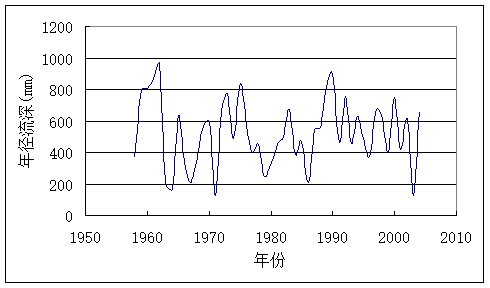
\includegraphics[width=0.7\textwidth]{3.png}
    \caption{年径流过程线图}
    \label{fig:annual_runoff_process}
\end{figure}
\subsubsection{洪水}
本流域及其周围附近均无实测流量资料,设计洪水采用暴雨资料推求。
\par
\textbf{设计暴雨}
设计暴雨选用距本工程最近的洞头站资料为代表,年最大暴雨系列为1957$\sim$2005共48年。洞头站年最大一日暴雨柱状图见图4,年最大三日暴雨柱状图见图5,实测大暴雨统计成果见表5。
% insert figure

\begin{figure}[h]
    \centering
    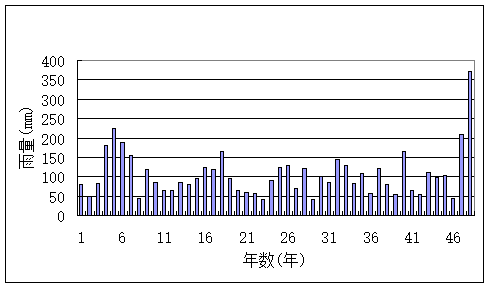
\includegraphics[width=0.7\textwidth]{4.png}
    \caption{洞头站1957$\sim$2005年年最大一日暴雨柱状图}
    \label{fig:annual_max_daily_rainfall}
\end{figure}
\begin{figure}[h]
    \centering
    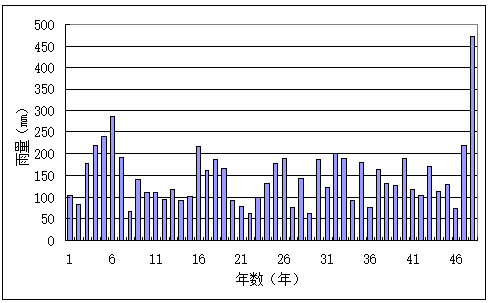
\includegraphics[width=0.7\textwidth]{5.png}
    \caption{年最大三日暴雨柱状图}
    \label{fig:annual_max_three_day_rainfall}
\end{figure}
\newpage

通过年最大暴雨频率分析,求得设计暴雨成果见表6(表中24小时雨量按一日雨量的1.13倍计)。年最大一日、三日暴雨频率曲线见附图 “洞黄围初-2-02”。
\begin{table}[h]
    \centering
    \caption{实测大暴雨统计成果}
    \resizebox*{0.8\textwidth}{!}{
    \begin{tabular}{|c|c|c|c|c|c|c|}
        \hline
        序号 & 一日雨量 (mm) & 发生年月 & 三日雨量 (mm) & 发生年月 & 七日雨量 (mm) & 发生年月 \\ \hline
        1 & 372.2 & 2005.7 & 472.5 & 2005.7 & 472.5 & 2005.7 \\ \hline
        2 & 225.8 & 1961.11 & 286.6 & 1962.9 & 348.5 & 1990.8 \\ \hline
        3 & 208.1 & 2004.8 & 240.8 & 1961.11 & 303.3 & 1962.9 \\ \hline
        4 & 189.5 & 1962.9 & 218.1 & 2004.8 & 298.2 & 1961.11 \\ \hline
        5 & 181.9 & 1960.9 & 217.8 & 1960.9 & 278.4 & 2004.8 \\ \hline
        6 & 166.1 & 1975.8 & 217.4 & 1973.10 & 248.0 & 1994.6 \\ \hline
        7 & 164.2 & 1997.8 & 201.4 & 1989.7 & 244.9 & 1960.9 \\ \hline
        8 & 154.6 & 1963.9 & 192.8 & 1963.9 & 241.7 & 1963.9 \\ \hline
        9 & 144.3 & 1989.7 & 191.2 & 1983.8 & 238.3 & 1987.9 \\ \hline
        10 & 129.5 & 1983.8 & 191.2 & 1997.8 & 223.9 & 1973.10 \\ \hline
    \end{tabular}
    }
    \label{tab:rainfall_statistics}
\end{table}

\begin{table}[h]
    \centering
    \caption{设计暴雨成果表}
    \begin{tabular}{|c|c|c|c|c|c|c|c|c|}
        \hline
        参数 & 均值 (mm) & Cv & Cs/Cv & 1\% & 2\% & 5\% & 10\% & 20\% \\ \hline
        一日雨量 & 106 & 0.58 & 3.5 & 329 & 286 & 229 & 186 & 143 \\ \hline
        24小时雨量 & 120 & 0.58 & 3.5 & 372 & 323 & 259 & 210 & 162 \\ \hline
        三日雨量 & 145 & 0.55 & 3.5 & 429 & 375 & 304 & 249 & 195 \\ \hline
    \end{tabular}
    \label{tab:design_rainfall_results}
\end{table}
设计暴雨成果比较见表7。由表7可见,本次设计暴雨成果要比可研阶段增大,其主要原因是本次设计增加了今年5号台风带来的特大暴雨,使暴雨统计参数发生了一定的变化。
\begin{table}[h]
    \centering
    \caption{设计暴雨成果比较表}
    \resizebox{0.6\textwidth}{!}{
    \begin{tabular}{|c|c|c|c|c|c|c|}
        \hline
        设计阶段 & 参数 & 1\% & 2\% & 5\% & 10\% & 20\% \\ \hline
        初设 & 24小时雨量 & 372 & 323 & 259 & 210 & 162 \\ \hline
        初设 & 三日雨量 & 429 & 375 & 304 & 249 & 195 \\ \hline
        可研 & 24小时雨量 & 268 & 241 & 205 & 176 & 146 \\ \hline
        可研 & 三日雨量 & 322 & 294 & 255 & 224 & 190 \\ \hline
        查图 & 24小时雨量 & 328 & 290 & 239 & 199 & 159 \\ \hline
        查图 & 三日雨量 & 424 & 374 & 308 & 257 & 205 \\ \hline
    \end{tabular}
    }
    \label{tab:design_rainfall_comparison}
\end{table}

\par \textbf{设计雨型}
\par
设计暴雨的日程分配为:最大24小时雨量位于3日雨量的第二日;其余2日雨量,第一日为3日雨量减去24小时雨量之差的60\%,第三日为3日雨量减去24小时雨量之差的40\%。
设计暴雨的时程分配,各时段雨量按暴雨公式计算,然后按《暴雨图集》雨型模式排位。其中,暴雨衰减指数取值为0.57$\sim$0.60。
\par \textbf{设计洪水}

\par
围区上游的山地面积大多位于黄岙一期,且山坡较陡,植被一般,又无溪流,暴雨降下后以坡面流的形式很快流入围区,故应用蓄满产流的简易扣损法直接计算产流过程。

鉴于流域内不同下垫面条件对降雨径流关系影响较大的客观规律,将区内分成山区、平原陆地及河网等三大地类计算产水过程。净雨计算采用以下扣损方案:

\begin{itemize}
    \item \textbf{山区}:
    \begin{itemize}
        \item 土壤最大含水量:$I_{max}=100$mm;
        \item 土壤前期含水量:75mm;
        \item 初损:25mm;
        \item 后损:0.5mm/h。
    \end{itemize}
    \item \textbf{平原陆地}:
    \begin{itemize}
        \item 最大持水深:240mm;
        \item 土壤前期含水量:204mm;
        \item 初损:36mm;
        \item 后损:0.5mm/h。
    \end{itemize}
    \item \textbf{河网}:
    \begin{itemize}
        \item 初损:0mm;
        \item 后损:0.2mm/h。
    \end{itemize}
\end{itemize}
\begin{table}[h]
    \centering
    \caption{黄岙二期围涂设计净雨成果表}
    \begin{tabular}{|c|c|c|c|c|c|}
        \hline
        项目 & 1\% & 2\% & 5\% & 10\% & 20\% \\ \hline
        三日毛雨 & 429 & 375 & 304 & 249 & 195 \\ \hline
        三日净雨 & 384.2 & 330.2 & 260 & 206.7 & 153.9 \\ \hline
    \end{tabular}
    \label{tab:three_day_rainfall}
\end{table}

\begin{table}[h]
    \centering
    \caption{黄岙二期围涂最大24小时设计净雨过程表}
    \resizebox{0.5\textwidth}{!}{ % 缩放表格以适应页面宽度
        \begin{tabular}{|c|c|c|c|c|c|c|}
            \hline
            时段 (h) & 1\% & 2\% & 5\% & 10\% & 20\% \\ \hline
            25 & 6.3 & 5.5 & 4.2 & 2.6 & 0.0 \\ \hline
            26 & 6.5 & 5.6 & 4.3 & 3.3 & 0.9 \\ \hline
            27 & 6.7 & 5.8 & 4.4 & 3.4 & 2.5 \\ \hline
            28 & 6.9 & 5.9 & 4.6 & 3.5 & 2.6 \\ \hline
            29 & 7.1 & 6.1 & 4.7 & 3.7 & 2.7 \\ \hline
            30 & 7.3 & 6.3 & 4.9 & 3.8 & 2.8 \\ \hline
            31 & 7.6 & 6.5 & 5.0 & 3.9 & 2.9 \\ \hline
            32 & 7.9 & 6.8 & 5.2 & 4.1 & 3.0 \\ \hline
            33 & 8.2 & 7.0 & 5.4 & 4.2 & 3.1 \\ \hline
            34 & 8.5 & 7.3 & 5.7 & 4.4 & 3.3 \\ \hline
            35 & 8.9 & 7.6 & 5.9 & 4.6 & 3.4 \\ \hline
            36 & 9.3 & 8.0 & 6.2 & 4.9 & 3.6 \\ \hline
            37 & 9.7 & 8.4 & 6.5 & 5.1 & 3.8 \\ \hline
            38 & 10.3 & 8.9 & 6.9 & 5.4 & 4.0 \\ \hline
            39 & 10.9 & 9.4 & 7.4 & 5.8 & 4.3 \\ \hline
            40 & 11.6 & 10.1 & 7.9 & 6.2 & 4.6 \\ \hline
            41 & 13.6 & 11.8 & 9.3 & 7.4 & 5.5 \\ \hline
            42 & 16.9 & 14.7 & 11.6 & 9.3 & 7.0 \\ \hline
            43 & 23.9 & 20.7 & 16.5 & 13.3 & 10.2 \\ \hline
            44 & 32.5 & 28.2 & 22.6 & 18.4 & 14.1 \\ \hline
            45 & 94.5 & 82.0 & 67.8 & 56.7 & 45.0 \\ \hline
            46 & 19.6 & 17.0 & 13.5 & 10.8 & 8.2 \\ \hline
            47 & 15.1 & 13.0 & 10.3 & 8.2 & 6.1 \\ \hline
            48 & 12.5 & 10.8 & 8.5 & 6.7 & 5.0 \\ \hline
        \end{tabular}
    }
    \label{tab:net_rainfall_results}
\end{table}
\newpage
\subsubsection{潮汐}

\subsubsection{潮汐特征}
本工程附近海区的潮汐,属正规半日潮。根据洞头潮位站实测资料统计:
\begin{itemize}
    \item 最高潮位:6.27m(1994年);
    \item 最低潮位:-1.77m(2004年);
    \item 多年平均高潮位:4.03m;
    \item 多年平均低潮位:-0.08m;
    \item 多年平均潮位:1.97m;
    \item 最大潮差:6.77m(1996年);
    \item 最小潮差:1.13m(1987年);
    \item 平均潮差:4.09m;
    \item 平均涨潮历时:6.17小时;
    \item 平均落潮历时:6.08小时。
\end{itemize}
\begin{table}[h]
    \centering
    \caption{潮汐特征值统计表}
    \begin{tabular}{|c|c|c|}
        \hline
        项目 & 特征值 & 备注 \\ \hline
        \multicolumn{3}{|c|}{潮位(m)} \\ \hline
        实测最高 & 6.27 & 1994年8月21日 \\ \hline
        实测最低 & -1.77 & 2004年4月6日 \\ \hline
        平均高 & 4.03 & \\ \hline
        其中大潮平均高 & 4.85 & \\ \hline
        其中小潮平均高 & 3.10 & \\ \hline
        平均低 & -0.08 & \\ \hline
        其中大潮平均低 & -0.98 & \\ \hline
        其中小潮平均低 & 1.07 & \\ \hline
        平均 & 1.97 & \\ \hline
        \multicolumn{3}{|c|}{潮差(m)} \\ \hline
        最大 & 6.77 & \\ \hline
        最小 & 1.13 & \\ \hline
        平均 & 4.09 & \\ \hline
        \multicolumn{3}{|c|}{历时(h)} \\ \hline
        涨潮 & 6.17 & \\ \hline
        落潮 & 6.08 & \\ \hline
    \end{tabular}
    \label{tab:tide_characteristics}
\end{table}
\subsubsection{设计潮位}
洞头潮位站自1984年开始观测,至2005 年已有22 年观测资料。
另与坎门站潮位相关分析,其相关系数为0.999,
可插补展延1958$\sim$1983年的潮位系列。
1958$\sim$2005年年最高潮位过程线见图6。







\begin{figure}[h]
    \centering
    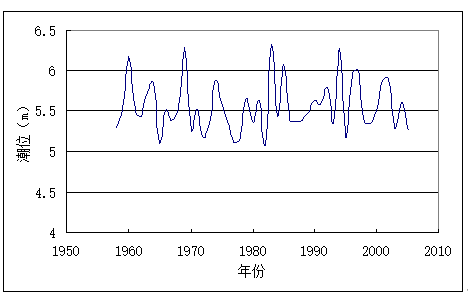
\includegraphics[width=0.5\textwidth]{7.png}
    \caption{1958$\sim$2005年年最高潮位过程线}
    \label{fig:annual_highest_tide_level}
\end{figure}
\subsubsection{龙口堵口潮型 }
采取常规的抛石合龙工艺, 对非汛期中最高潮位进行频率分析计算,取5 年一遇非汛期设计高潮位5.50m 为设计标准,
从实测资料中选取龙口堵口水力计算的典型潮型,详见表11。龙口堵口设计潮位过程线见图。
\begin{figure}[h]
    \centering
    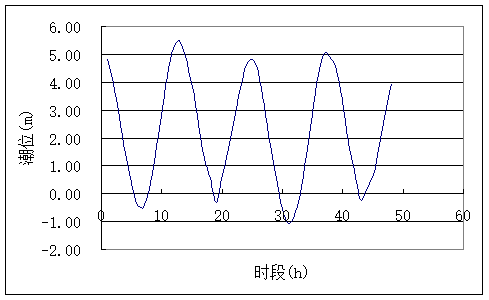
\includegraphics[width=0.6\textwidth]{8.png}
    \caption{龙口堵口设计潮位过程线}
    \label{fig:dragon_port_tide_level}
    
\end{figure}

\begin{table}[h]
    \centering
    \caption{围堤堵口设计潮位过程表}
    \resizebox{0.4\textwidth}{!}{
    \begin{tabular}{|c|c|c|c|}
        \hline
        时段(h) & 潮位(m) & 时段(h) & 潮位(m) \\ \hline
        1 & 4.81 & 25 & 4.8 \\ \hline
        2 & 3.99 & 26 & 4.34 \\ \hline
        3 & 2.79 & 27 & 3.18 \\ \hline
        4 & 1.44 & 28 & 1.73 \\ \hline
        5 & 0.42 & 29 & 0.53 \\ \hline
        6 & -0.38 & 30 & -0.53 \\ \hline
        7 & -0.48 & 31 & -1.06 \\ \hline
        8 & 0.16 & 32 & -0.77 \\ \hline
        9 & 1.37 & 33 & -0.04 \\ \hline
        10 & 2.80 & 34 & 1.37 \\ \hline
        11 & 4.21 & 35 & 2.85 \\ \hline
        12 & 5.20 & 36 & 4.23 \\ \hline
        13 & 5.50 & 37 & 5.04 \\ \hline
        14 & 4.92 & 38 & 4.87 \\ \hline
        15 & 3.84 & 39 & 4.46 \\ \hline
        16 & 2.47 & 40 & 3.39 \\ \hline
        17 & 1.30 & 41 & 1.89 \\ \hline
        18 & 0.55 & 42 & 0.87 \\ \hline
        19 & -0.32 & 43 & -0.21 \\ \hline
        20 & 0.67 & 44 & 0.13 \\ \hline
        21 & 1.61 & 45 & 0.68 \\ \hline
        22 & 2.71 & 46 & 1.76 \\ \hline
        23 & 3.77 & 47 & 2.9 \\ \hline
        24 & 4.59 & 48 & 3.97 \\ \hline
    \end{tabular}
    }
    \label{tab:dragon_port_tide_process}
\end{table}
\newpage
\newpage
\subsubsection{波浪}
\textbf{计算方法}
\par
黄岙围涂工程位于大门岛南侧,以青菱屿为界,分为东西两侧,其中东侧白马堤较短,长约700m,西侧下乌仙堤较长,因水深变化较大,可再分为下乌仙堤西段与下乌仙堤东段,
东西段长均为1600m 左右。根据黄岙围涂周围海域和波浪资料情况,
白马堤和下乌仙堤分别采用不同的方法计算堤前波要素。
其中下乌仙堤采用风推浪方法计算,白马堤采用浪推浪方法计算。


\par

\par
\textbf{破碎波高}
\par
由《海港水文规范》知,当海堤坡度$i <= 1/200$ ,破碎波高可按下式计算。

\begin{equation}
    H_b = \gamma_b \times h_b
\end{equation}

\begin{itemize}
    \item $\gamma_b$ —— 破碎指标,取 $\gamma_b = 0.60$;
    \item $h_b$ —— 水深,单位:$\text{m}$;
    \item $H_b$ —— 破碎波高,单位:$\text{m}$。
\end{itemize}

\par
\textbf{累计频率为1\%时爬高值}

\par

根据设计规范(如《海堤工程设计规范》或《港口与航道水文规范》),爬高值 $R_0$ 的计算公式可能如下:

\begin{equation}
    R_0 = \alpha \cdot H_{1\%} \cdot \beta
\end{equation}

\begin{itemize}
    \item $\alpha$:与波浪特性和堤坡有关的系数;
    \item $\beta$:与堤前水深和波浪周期有关的修正系数。
\end{itemize}



\par
\textbf{不同累计频率下的波高}
\par

累计频率的波高换算可以按《海港水文规范》式(4.2.2)计算:
\begin{equation}
    H_F = \bar{H} \left[ 
    \frac{4}{\pi} \left( 1 + \frac{1}{\sqrt{2\pi}} H^* \right) \ln F 
    \right]^{1 - \frac{H^*}{2}}
\end{equation}

\begin{itemize}
    \item $\bar{H}$ —— 平均波高,单位:$\text{m}$;
    \item $H^*$ —— 相对水深,$H^* = \frac{\bar{H}}{d}$,单位:$\text{m}$;
    \item $F$ —— 累积频率;
    \item $d$ —— 水深,单位:$\text{m}$;
    \item $H_F$ —— 相应的累计算频率的波高,单位:$\text{m}$。
\end{itemize}



\par



\textbf{波浪计算}

\par


\par(1)下乌仙堤
\par
下乌仙堤设计波浪要素采用《浙江省海塘工程技术规定》(1999年9月5日发布,以下简称“规定”)中的方法计算。设计风速查读“规定”中的风速均值等值线图和风速变差系数Cv等值线图,由其风向、风区内的风速均值、风速变差系数Cv,按“规定”方法求得10分钟设计风速。风区平均计算水深为风区平均水深加上设计频率高潮位求得
\par
根据风场要素,采用“莆田海堤试验站公式”计算波浪要素。
莆田海堤试验站公式如下:
\begin{equation}
    \frac{g\bar{H}}{V^2} = 0.13 th \left[ 0.7 \left( \frac{g d}{V^2} \right)^{0.7} th \left\{ 
    \frac{0.0018 \left( \frac{g F}{V^2} \right)^{0.45}}{0.13 th \left[ 0.7 \left( \frac{g d}{V^2} \right)^{0.7} \right]} 
    \right\} \right]
    \label{eq:wave_height}
\end{equation}

\begin{equation}
    \frac{gT}{V} = 13.9 \left( \frac{g\bar{H}}{V^2} \right)^{0.5}
    \label{eq:wave_period}
\end{equation}

式中:
\begin{itemize}
    \item $g$ —— 重力加速度($9.81\,\text{m/s}^2$);
    \item $F$ —— 风区长度($m$);
    \item $V$ —— 设计风速($m/s$);
    \item $d$ —— 风区平均计算水深($m$);
    \item $\bar{H}$ —— 平均波高($m$);
    \item $\bar{T}$ —— 平均波周期($s$)。
\end{itemize}
\par
(2)白马堤
\par
白马堤采用《浙江省海塘工程技术规定》中的浪推浪方法计算。
主要依据资料为浙南南麂站深水设计波要素。南麂站E$\sim$ESE向 50年一遇平均波高5.0m,平均波周期13.4s,深水波长280.1m。
通过波浪浅水变形计算,求得堤前设计波要素见表12。

\begin{table}[h]
    \centering
    \small
    \caption{堤段设计波浪要素表}
    \resizebox{0.6\textwidth}{!}{ % 缩放表格以适应页面宽度
        \begin{tabular}{|c|c|c|c|}
            \hline
            堤段 & 下乌仙西堤 & 下乌仙东堤 & 白马堤 \\ \hline
            风向 & S$\sim$SSW & S$\sim$SSW & E$\sim$ESE \\ \hline
            设计风速(m/s) & 38.8 & 38.8 & 浪推浪 \\ \hline
            设计潮位(m) & 6.78 & 6.78 & 6.78 \\ \hline
            平均波高(m) & 1.39 & 1.41 & 2.1 \\ \hline
            平均波周期(s) & 5.2 & 5.3 & 13.4 \\ \hline
            波长(m) & 42.6 & 43.4 & 131.4 \\ \hline
            设计波高(F=1\%) & 3.04 & 3.07 & 4.4 \\ \hline
            设计波高(F=2\%) & 2.84 & 2.87 & 4.13 \\ \hline
            设计波高(F=5\%) & 2.53 & 2.56 & 3.71 \\ \hline
            设计波高(F=13\%) & 2.14 & 2.17 & 3.18 \\ \hline
            破碎波高(m) & 4.65 & 4.65 & 5.73 \\ \hline
        \end{tabular}
    }
    \label{tab:wave_elements}
\end{table}


\par
\textbf{设计波要素和设计潮位}
\par
温州市洞头区黄岙二期围涂工程白马堤定位为Ⅲ级海塘工程,设计高潮位取 50 年一遇
重现期。

洞头区观测 1985$\sim$2000 年共 16 年潮位资料,尚不足 20 年,需通过相关关系插补潮位资料。经分析玉环县坎门站与洞头站潮汐特征相似,
故取坎门站作为参证站。根据相关关系插补洞头站 1980$\sim$1985 年 6 年最高潮位(考虑到洞头站 1985 年初次观测,该年观测最高潮位与周围测站成果存在极不协调性,故该年亦采用相关式进行插补),将 1980$\sim$1985 年插补资料与 1986$\sim$2000 年洞头站实测最高潮位值进行频率分析,采用 P-Ⅲ 型曲线进行拟合,求得洞头站 50 年一遇设计高潮位为 6.89m(洞头基准)。
龙口度汛的设计高潮位取为6.27m,堵口合龙的设计高潮位为5.04m。

设计波浪标准包括设计波高的波列累积频率标准和重现期标准。对于不同的计算内
容应采用不同的设计波浪标准。波浪的设计重现期与设计高潮位的重现期相同,为 50
年一遇。
因本围涂工程所在区域及附近没有波浪实测资料,故波浪计算只能根据风场要素进
行推算,风速的重现期即为波浪的重现期,风向组的平均方向即为波向。


\section{平面布置}
\subsection{布置原则}
\par
\begin{enumerate}
    \item 根据围涂工程开发目标与规划规模,计划围涂 4260 亩,其中 1000 亩用于房地产开发,3260 亩用于海水养殖;
    \item 堤线的平面布置应顺直,避免曲折过多、凹凸多变导致波能集中;
    \item 综合考虑利用地形地质条件,减少工程量;
    \item 选取对防浪有利的方向,尽可能避免堤线与强风向、强浪向正交。
\end{enumerate}

\subsection{堤线布置}
根据以上布置原则
堤线自下乌仙咀开始,下乌仙西堤A1(3092841.265,537309.516)与A2(3092633.598,538905.682)之间的距离约为1.8km;
下乌仙东堤A2与A3(3092176.099,540443.220)之间的距离约为1.4km;
白马堤A4(3092194.584,540733.291)与A5(3092351.400,541417.619)之间的距离约为0.8km;
\par
围堤布置方案一方面保证了规划的围涂面积,满足发展需求,另一方面充分利用了
已有地形地貌,保持堤线顺直,减少了工程量,此外还尽量避免与
强浪向正交。

堤线总长度为4km,其中下乌仙堤长度为3.2km,白马堤长度为0.8km。
具体堤线布置如图8所示:
\begin{figure}[h]
    \centering
    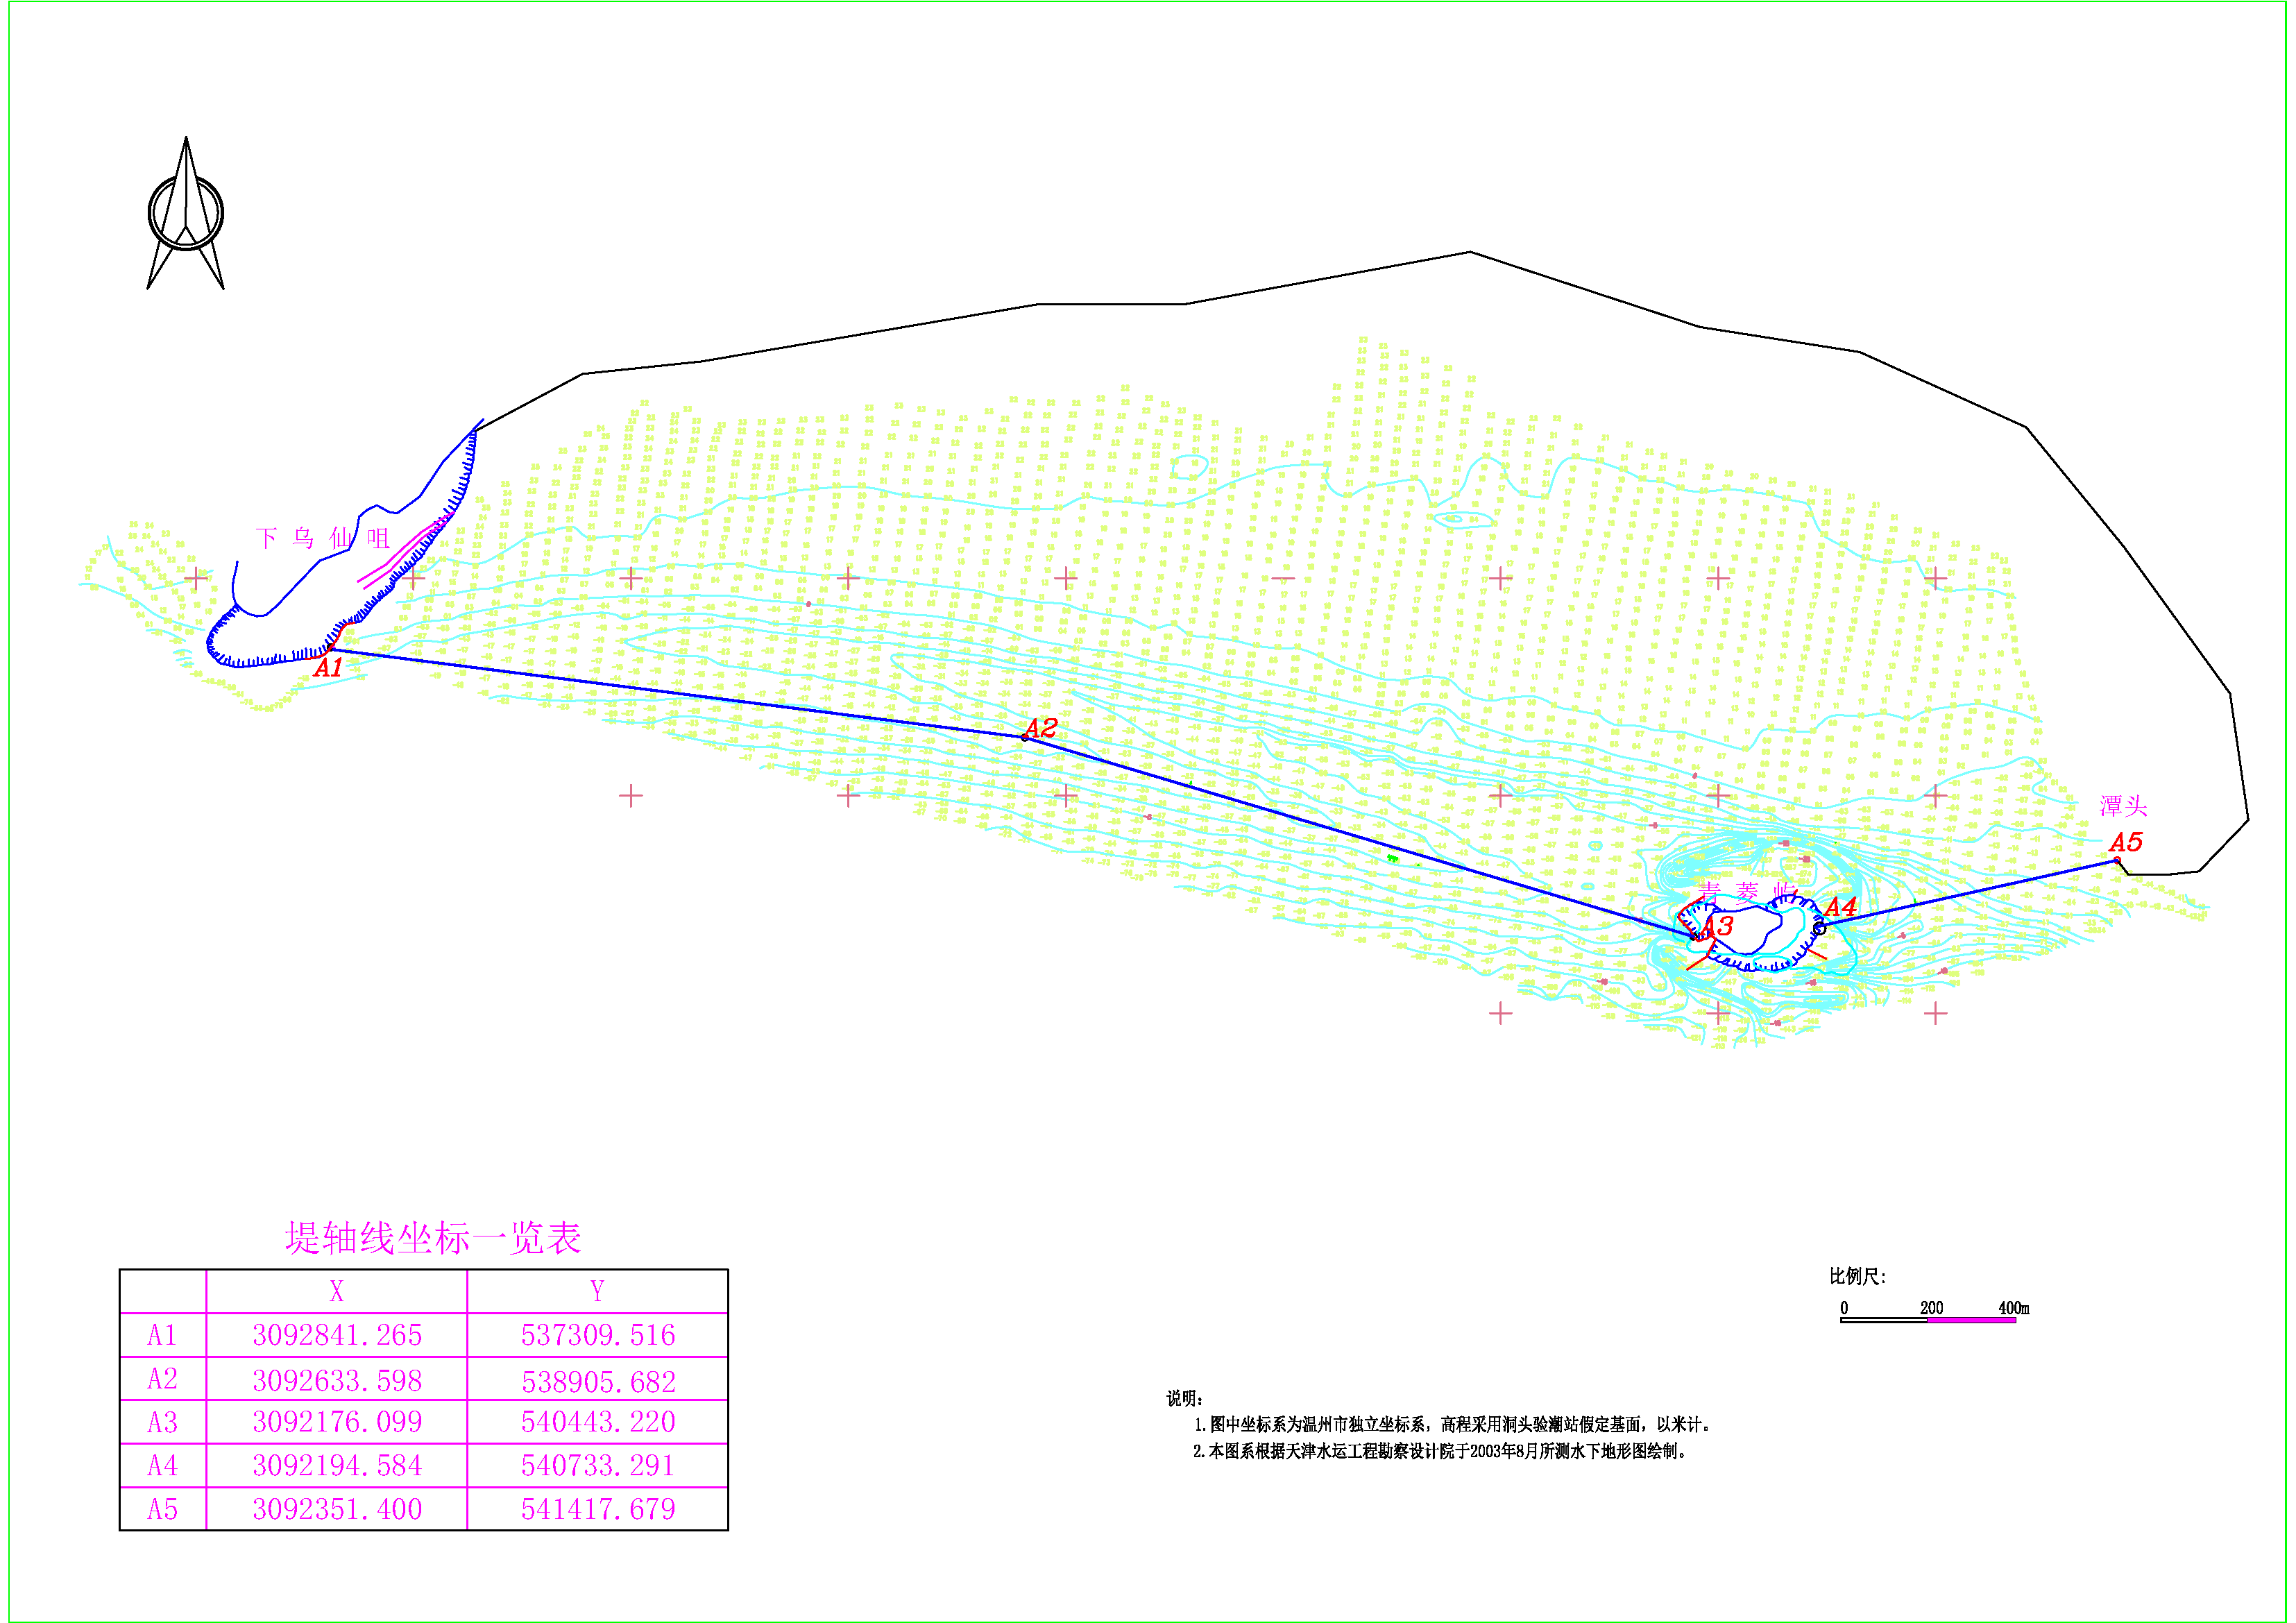
\includegraphics[width=0.8\textwidth]{10.png}
    \caption{堤线布置图}
    \label{fig:sea_dike_layout}
\end{figure}
\section{海堤设计}

由于本次毕业设计分配工程区域为 白马堤,故接下来主要针对白马堤进行设计。
\subsection{海堤断面型式方案比较}
考虑到围涂造地区域的地基土强度较弱,容易引起较大的地基沉降,拟设计两种海堤的断面方案,分别为斜坡式海堤和混合式海堤两种形式。斜坡式海堤和混合式海堤方案均采用土石混合堤,均设消浪平台,用以消弱波浪的爬高能力。
选取下乌仙堤A2处作为典型断面,设计两套方案。
\par
\textbf{堤顶高程的确定}
\par
\begin{itemize}
    \item[1] 波浪爬高计算
\end{itemize}
根据设计规范计算波浪爬高,计算公式如下:

\begin{equation}
    R_F = K_\Delta K_v R_0 H_{1\%} K_F
\end{equation}

式中:
\begin{itemize}
    \item $K_\Delta$ —— 粒滞系数;
    \item $K_v$ —— 与风速及堤前水深有关的系数;
    \item $R_0$ —— 累计频率为 1\% 时的爬高值;
    \item $H_{1\%}$ —— 波高累计频率为 1\% 的波高值,当 $H_{1\%} > H_b$ 时,则 $H_{1\%}$ 取 $H_b$;
    \item $K_F$ —— 爬高累计频率换算系数,$K_F = 0.74$;
\end{itemize}

\par
\textbf{下乌仙堤A2}
\par
堤前水深d = 1.6m;
\par
\begin{table}[h]
    \centering
    \caption{波浪爬高计算参数与结果}
    \begin{tabular}{|c|c|c|}
        \hline
        参数符号 & 参数名称 & 取值 \\ \hline
        $k_\Delta$ & 粒滞系数 & 0.5230 \\ \hline
        $H_{1\%}$ & 波高累计频率为 1\% 的波高值 & 3.04\,m \\ \hline
        $k_\beta$ & 波浪入射角修正系数 & 1.00 \\ \hline
        $k_\gamma$ & 水深修正系数 & 1.00 \\ \hline
        $k_v$ & 风速及堤前水深修正系数 & 1.284 \\ \hline
        $R_0$ & 累计频率为 1\% 时的爬高值 & 1.51 \\ \hline
        $k_F$ & 爬高累计频率换算系数 & 0.74 \\ \hline
        $R_F$ & 波浪爬高计算结果 & $0.523 \cdot 1.284 \cdot 1.51 \cdot 3.04 \cdot 0.74 = 2.28\,\text{m}$ \\ \hline
    \end{tabular}
    \label{tab:wave_runup_calculation}
\end{table}

\par

当上部陡墙坡度小于等于 0.4 时,波浪爬高采用以下公式计算
\begin{equation}
    R_{F\%} = 1.36 \left( 1.5 H K_z \tanh \frac{2 \pi d}{L} - dw \right) k_y \cdot k_v
\end{equation}

式中:
\begin{itemize}
    \item $d$ —— 堤前水深,单位:$\text{m}$;
    \item $L$ —— 波长,单位:$\text{m}$;
    \item $dw$ —— 平台位于水下时取正值,平台高程为 $4.50\,\text{m}$,$dw = 0.2\,\text{m}$;
    \item $H$ —— 允许越浪时的累积频率的波高;
    \item $K_z$ —— 系数,根据 $\zeta = \left( \frac{d_w}{d} \right) \left( \frac{d}{H} \right) \tanh \frac{2 \pi d}{L}$,查《浙江省海塘技术规定(上)》图 5.2.5-2 确定;
    \item $k_y$ —— 修正系数;
    \item $k_v$ —— 风速及堤前水深修正系数。
\end{itemize}

\par

\textbf{下乌仙堤A2}

\par
堤前水深d = 1.6m
\par

\begin{table}[h]
    \centering
    \caption{波浪爬高计算参数与结果}
    \begin{tabular}{|c|c|c|}
        \hline
        参数符号 & 参数名称 & 取值 \\ \hline
        $K_z$ & 系数 & 1.40 \\ \hline
        $H_{13\%}$ & 波高累计频率为 13\% 的波高值 & 2.17\,m \\ \hline
        $dw$ & 平台高程 & 0.2\,m \\ \hline
        $k_y$ & 修正系数 & 1.0 \\ \hline
        $k_v$ & 风速及堤前水深修正系数 & 1.284 \\ \hline
        $d$ & 堤前水深 & 1.6\,m \\ \hline
        $L$ & 波长 & 42.6\,m \\ \hline
        $R_{13\%}$ & 波浪爬高计算结果 & $1.36 \cdot \left( 1.50 \cdot 2.17 \cdot 1.40 \cdot \tanh \frac{2 \pi \cdot 1.6}{42.6} - 0.2 \right) \cdot 1.0 \cdot 1.284 = 1.49\,\text{m}$ \\ \hline
    \end{tabular}
    \label{tab:wave_runup_calculation}
\end{table}


\begin{itemize}
    \item [2] 防浪墙顶高程的确定
\end{itemize}
由《海堤工程设计规范》得,防浪墙顶高程的计算公式如下:
\begin{equation}
    Z_p = h_p + R_{F\%} + \Delta h
\end{equation}

\begin{itemize}
    \item $Z_p$ —— 防浪墙顶高程;
    \item $h_p$ —— 设计频率的高潮位,为 $6.89\,\text{m}$;
    \item $R_{F\%}$ —— 波浪爬高,斜坡堤为 $2.28\,\text{m}$,混合式海堤为 $1.49\,\text{m}$;
    \item $\Delta h$ —— 安全加高值,取 $0.50\,\text{m}$。
\end{itemize}



由上述计算过程可以得到A2处:

斜坡式海堤的防浪墙的顶高程为$6.89+2.28+0.5 = 8.22\textbf{m} $

混合式海堤的防浪墙的顶高程为 $6.89+1.49+0.5=7.93\textbf{m}$。

\begin{itemize}
    \item [3] 堤顶高程的确定
\end{itemize}
海堤的堤顶高程应同时满足大于设计一般高潮位 ,以此计算海堤堤顶
高程和堤顶路面高程的取值见表


\begin{table}[h]
    \centering
    \caption{斜坡堤设计参数与计算结果}
    \resizebox{0.5\textwidth}{!}{
    \begin{tabular}{|c|c|c|c|}
        \hline
        堤段 & 下乌仙堤A1 & 下乌仙堤A2 & 下乌仙堤A3 \\ \hline
        波向 & $S-SSW$ & $S-SSW$ & $S-SSW$ \\ \hline
        波浪性质 &  风推浪 & 风推浪 & 风推浪 \\ \hline
        重现期 & 200年 & 200年 & 200年 \\\hline
        设计潮位 $h_p$ (m) & 6.89 & 6.89 & 6.89 \\ \hline
        设计风速 $V$ (m/s) & 38.8 & 38.8 & 38.8 \\ \hline
        平均波高 $\bar{H}$ (m) & 1.39 & 1.40 & 1.41 \\ \hline
        平均波周期 $\bar{T}$ (s) & 5.2 & 5.2 & 5.3 \\ \hline
        设计波长 $L$ (m) & 42.6 & 43.0 & 43.4 \\ \hline
        设计波高 $H_{1\%}$ (m) & 3.04 & 3.05 & 3.07 \\ \hline
        设计波高 $H_{13\%}$ (m) & 2.14 & 2.15 & 2.17 \\ \hline
        粒滞系数 $K_\Delta$ & 0.523 & 0.523 & 0.523 \\ \hline
        波向修正系数 $K_\beta$ & 1 & 1 & 1 \\ \hline
        压载系数 $K_y$ & 1 & 1 & 1 \\ \hline
        波浪爬高值 $R_{13\%}$ (m) & 1.45 & 1.49 & 1.45 \\ \hline
        安全加高值 $\Delta h$ (m) & 0.5 & 0.5 & 0.5 \\ \hline
        爬高计算防浪墙顶高程 (m) & 8.05 & 8.22 & 8.20 \\ \hline
        $h_p  + 0.5H_{1\%}$ &8.89&8.90&8.89 \\ \hline
        设计防浪墙顶高程 (m) & 9.0 & 9.0 &9.0 \\ \hline
        有效越浪量 (m\textsuperscript{3}/s·m) & 0.00311 & 0.00364 & 0.00311 \\ \hline
        设计堤顶高程 (m) & 9.0 & 9.5 & 9.0 \\ \hline
    \end{tabular}
    }
    \label{tab:design_parameters}
\end{table}



\begin{table}[h]
    \centering
    \caption{混合堤设计参数与计算结果}
    \resizebox{0.5\textwidth}{!}{
    \begin{tabular}{|c|c|c|c|}
        \hline
        堤段 & 下乌仙堤A1 & 下乌仙堤A2 & 下乌仙堤A3 \\ \hline
        波向 & $S-SSW$ & $S-SSW$ & $S-SSW$ \\ \hline
        波浪性质 &  风推浪 & 风推浪 & 风推浪 \\ \hline
        重现期 & 200年 & 200年 & 200年 \\\hline
        设计潮位 $h_p$ (m) & 6.89 & 6.89 & 6.89 \\ \hline
        设计风速 $V$ (m/s) & 38.8 & 38.8 & 38.8 \\ \hline
        平均波高 $\bar{H}$ (m) & 1.39 & 1.40 & 1.41 \\ \hline
        平均波周期 $\bar{T}$ (s) & 5.2 & 5.2 & 5.3 \\ \hline
        设计波长 $L$ (m) & 42.6 & 43.0 & 43.4 \\ \hline
        设计波高 $H_{1\%}$ (m) & 3.04 & 3.05 & 3.07 \\ \hline
        设计波高 $H_{13\%}$ (m) & 2.14 & 2.15 & 2.17 \\ \hline
        粒滞系数 $K_\Delta$ & 0.523 & 0.523 & 0.523 \\ \hline
        波向修正系数 $K_\beta$ & 1 & 1 & 1 \\ \hline
        压载系数 $K_y$ & 1 & 1 & 1 \\ \hline
        波浪爬高值 $R_{13\%}$ (m) & 1.45 & 1.49 & 1.45 \\ \hline
        安全加高值 $\Delta h$ (m) & 0.5 & 0.5 & 0.5 \\ \hline
        爬高计算防浪墙顶高程 (m) & 7.55 & 7.93 & 7.20 \\ \hline
        $h_p  + 0.5H_{1\%}$ &8.89&8.90&8.89 \\ \hline
        设计防浪墙顶高程 (m) & 9.0 & 9.0 &9.0 \\ \hline
        有效越浪量 (m\textsuperscript{3}/s·m) & 0.00311 & 0.00364 & 0.00311 \\ \hline
        设计堤顶高程 (m) & 9.0 & 9.5 & 9.0 \\ \hline
    \end{tabular}
    }
    \label{tab:design_parameters}
\end{table}

\newpage
\newpage
\par
\subsubsection{海堤方案的护面处理}

A2处,200 年一遇设计高潮位值为 6.89m,为有效降低波浪爬高,采用
扭王字块体作为斜坡式防坡堤和混合式防坡堤护面块体。消浪平台设置在 5.00m
高程处,消浪平台前后边坡根据海堤规范,取 1:2,分别连接堤顶道路和缓坡。
混合式海堤斜坡式海堤的消浪平台设置在 4.50m 高程处,边坡坡度取用 1:3。
\begin{itemize}
    \item [1] 扭王块体稳定重量分析
\end{itemize}



\begin{equation}
    Q = 0.1 \frac{\gamma_b H^3}{K_D \left( \frac{\gamma_b}{\gamma} - 1 \right)^3 m}
\end{equation}

\begin{itemize}
    \item $Q$ —— 扭王字块体稳定重量;
    \item $\gamma_b$ —— 块石重度,取当地石料的建议重度 $26.0\,\text{kN/m}^3$;
    \item $\gamma$ —— 水重度,$9.81\,\text{kN/m}^3$;
    \item $H$ —— 设计波高,单位:$\text{m}$;
    \item $K_D$ —— 稳定系数,取中值为 $21$;
    \item $m$ —— 斜坡坡比;
    \item $\bar{H}/d < 0.3$ 时宜采用 $H_{5\%}$,$\bar{H}/d \geq 0.3$ 时宜采用 $H_{13\%}$。
\end{itemize}
下乌仙堤A2扭王块体稳定重量计算:

堤前水深$d:1.6\textbf{m}$
 
平均波高$\bar{H}:6.89\textbf{m}$

平均波高与水深比值$\bar{H}/d:4.31 > 0.3$ , 采用$H_{13\%}$

斜坡式海堤方案扭王块体重量计算:

已知参数:
\begin{itemize}
    \item $K_D = 21$,稳定系数;
    \item $m = 2.0$,斜坡坡比;
    \item $H_{13\%} = 2.15\,\text{m}$(A2);
    \item $\gamma_b = 23.0\,\text{kN/m}^3$,块石重度。
\end{itemize}

根据公式:
\begin{equation}
    Q = 0.1 \cdot \frac{\gamma_b H^3}{K_D \left( \frac{\gamma_b}{\gamma} - 1 \right)^3 \cdot m}
\end{equation}

代入数据:
\[
    Q = 0.1 \cdot \frac{23.0 \cdot 2.15^3}{21 \cdot \left( \frac{23.0}{9.81} - 1 \right)^3 \cdot 2.0}
\]

计算得:
\[
    Q = 0.25\,\text{t}
\]
混合式海堤方案扭王块体重量计算:

已知参数:

\begin{itemize}
    \item $K_D = 21$,稳定系数;
    \item $m = 3.0$,斜坡坡比;
    \item $H_{13\%} = 2.17\,\text{m}$(A2);
    \item $\gamma_b = 23.0\,\text{kN/m}^3$,块石重度。
\end{itemize}


根据公式:
\begin{equation}
    Q = 0.1 \cdot \frac{\gamma_b H^3}{K_D \left( \frac{\gamma_b}{\gamma} - 1 \right)^3 \cdot m}
\end{equation}

代入数据:
\[
    Q = 0.1 \cdot \frac{23.0 \cdot 2.17^3}{21 \cdot \left( \frac{23.0}{9.81} - 1 \right)^3 \cdot 3.0}
\]

计算得:
\[
    Q = 0.15\,\text{t}
\]

\textbf{由上述计算过程可以得到下乌仙堤A2点处,斜坡式海堤的扭王块体稳定重量为
0.25t, 混合式海堤的扭王块体稳定重量为 0.15t。}


\begin{itemize}
    \item [2] 扭王块体厚度计算
\end{itemize}
\par
依据《海堤工程设计规范》 ,扭王字块体的厚度计算公式:
\begin{equation}
    t = nC \left( \frac{Q}{0.1 \gamma_b} \right)^{\frac{1}{3}}
\end{equation}

式中:
\begin{itemize}
    \item $t$ —— 块体或块石护面层厚度;
    \item $n$ —— 护面块体或块石的层数,$n$ 为 1;
    \item $C$ —— 系数,按规范表 J.0.6-2 确定,为 1.36;
    \item $Q$ —— 块体或块石的稳定重量;
    \item $\gamma_b$ —— 块石重度。
\end{itemize}

\par

斜坡式海堤扭王块体护面厚度计算:


已知参数:
\begin{itemize}
    \item $C = 1.36$,系数;
    \item $Q = 0.25\,\text{t}$,块体稳定重量;
    \item $\gamma_b = 23.0\,\text{kN/m}^3$,块石重度;
    \item $n = 1.0$,护面块体的层数。
\end{itemize}

根据公式:
\begin{equation}
    t = nC \left( \frac{Q}{0.1 \gamma_b} \right)^{\frac{1}{3}}
\end{equation}

代入数据:
\[
    t = 1.0 \times 1.36 \times \left( \frac{0.25}{0.1 \times 23.0} \right)^{\frac{1}{3}}
\]

计算得:
\[
    t = 1.0 \times 1.36 \times \left( \frac{0.25}{2.3} \right)^{\frac{1}{3}} = 1.0 \times 1.36 \times (0.11)^{\frac{1}{3}} = 0.65\,\text{m}
\]

混合式海堤扭王块体护面厚度计算:



已知参数:
\begin{itemize}
    \item $C = 1.36$,系数;
    \item $Q = 0.15\,\text{t}$,块体稳定重量;
    \item $\gamma_b = 23.0\,\text{kN/m}^3$,块石重度;
    \item $n = 1.0$,护面块体的层数。
\end{itemize}

根据公式:
\begin{equation}
    t = nC \left( \frac{Q}{0.1 \gamma_b} \right)^{\frac{1}{3}}
\end{equation}

代入数据:
\[
    t = 1.0 \times 1.36 \times \left( \frac{0.15}{0.1 \times 23.0} \right)^{\frac{1}{3}}
\]


计算得:
\[
    t = 1.0 \times 1.36 \times \left( \frac{0.15}{2.3} \right)^{\frac{1}{3}} = 1.0 \times 1.36 \times (0.07)^{\frac{1}{3}} = 0.56\,\text{m}
\]



\textbf{由上述计算过程可以得到下乌仙堤A2点处,斜坡式海堤的扭王块体护面厚度为
0.65m, 混合式海堤的扭王块体护面厚度为 0.56m。}

\begin{itemize}
    \item [3] 扭王块体的数量计算
\end{itemize}

\begin{equation}
    N = AnC (1 - P') \left( \frac{0.1 \gamma_b}{Q} \right)^{\frac{2}{3}}
\end{equation}

式中:
\begin{itemize}
    \item $N$ —— 混凝土异型块体个数;
    \item $A$ —— 垂直于厚度的护面层平均面积;
    \item $P'$ —— 护面层的空隙率,扭王块取为 $50\%$;
    \item $\gamma_b$ —— 块石重度,取当地石料的重度 $26.0\,\text{kN/m}^3$;
    \item $Q$ —— 块石稳定重量。
\end{itemize}

斜坡式海堤扭王块体个数计算:
已知参数:
\begin{itemize}
    \item $A = 100.0\,\text{m}^2$,护面层平均面积;
    \item $C = 1.36$,系数;
    \item $P' = 50\%$,护面层空隙率;
    \item $\gamma_b = 23.0\,\text{kN/m}^3$,块石重度;
    \item $Q = 0.65\,\text{t}$,块体稳定重量。
\end{itemize}

根据公式:
\begin{equation}
    N = A n C (1 - P') \left( \frac{0.1 \gamma_b}{Q} \right)^{\frac{2}{3}}
\end{equation}

代入数据:
\[
    N = 100 \times 1 \times 1.36 \times (1 - 50\%) \left( \frac{0.1 \times 23.0}{0.65} \right)^{\frac{2}{3}}
\]
计算得:
\[
    N = 100 \times 1.36 \times 0.5 \times \left( \frac{2.3}{0.65} \right)^{\frac{2}{3}} \approx 100 \times 1.36 \times 0.5 \times 3.53 \approx 239.68
\]

最终结果:
\[
N \approx 239.68
\]
混合式海堤扭王块体个数计算:

已知参数:
\begin{itemize}
    \item $A = 100.0\,\text{m}^2$,护面层平均面积;
    \item $C = 1.36$,系数;
    \item $P' = 50\%$,护面层空隙率;
    \item $\gamma_b = 23.0\,\text{kN/m}^3$,块石重度;
    \item $Q = 0.56\,\text{t}$,块体稳定重量。
\end{itemize}

根据公式:
\begin{equation}
    N = A n C (1 - P') \left( \frac{0.1 \gamma_b}{Q} \right)^{\frac{2}{3}}
\end{equation}

代入数据:
\[
    N = 100 \times 1 \times 1.36 \times (1 - 50\%) \left( \frac{0.1 \times 23.0}{0.56} \right)^{\frac{2}{3}}
\]

计算得:
\[
    N = 100 \times 1.36 \times 0.5 \times \left( \frac{2.3}{0.56} \right)^{\frac{2}{3}} \approx 100 \times 1.36 \times 0.5 \times 4.54 \approx 308.72
\]

最终结果:
\[
N \approx 308.72
\]




\textbf{经计算得出下乌仙堤A2点处,斜坡式海堤坡面护面块石扭王块体个数为 240 个, 混合
式海堤坡面护面块石的扭王块体个数为 309 个。}
\par
\subsubsection{整体稳定性计算}
\begin{equation}
    K = \frac{\sum \left( c_i L_i + W_i \cos \alpha_i \tan \varphi_i \right) + T}{\sum W_i \sin \alpha_i}
\end{equation}
\begin{itemize}
        \item $K$ —— 抗滑安全系数;
        \item $W_i$ —— 土条的滑弧长、重量(kN);
        \item $L_i$ —— 土条的滑弧长(m);
        \item $c_i$ —— 土条滑动面上的凝聚力(kPa);
        \item $\varphi_i$ —— 土条滑动面上的内摩擦角(度);
        \item $\alpha_i$ —— 滑动面中点的切线与水平线的夹角(度);
        \item $T$ —— 土工织物设计强度(kN)。
\end{itemize}

经计算分析,

斜坡式海堤外坡稳定安全系数为 1.4;

内坡的稳定安全系数为 2.5;

混合式海堤外坡稳定安全系数为 1.4;

内坡的稳定安全系数为 2.4。

因此,两种设计海堤断面均满足的最小稳定安全系数满足规范要求。
各海堤典型断面稳定计算过程如下:



\newpage
\begin{table}[h]
    \centering
    \caption{海堤稳定性计算方法}
    \begin{tabular}{|c|c|}
        \hline
        \textbf{参数} & \textbf{取值} \\ \hline
        采用规范 & 通用方法 \\ \hline
        计算目标 & 安全系数计算 \\ \hline
        滑裂面形状 & 圆弧滑动法 \\ \hline
        海啸地震状况 & 不考虑地震 \\ \hline
    \end{tabular}
    \label{tab:stability_parameters}
\end{table}

\begin{table}[h]
    \centering
    \caption{稳定性计算条件}
    \begin{tabular}{|c|c|}
        \hline
        \textbf{圆弧稳定分析方法} & \textbf{瑞典条分法} \\ \hline
        土条重切向分力与滑动方向反向时 & 当下滑力对待 \\ \hline
        稳定计算目标 & 自动搜索最危险滑裂面 \\ \hline
        条分法的土条宽度(m) & 1.000 \\ \hline
        搜索时的圆心步长(m) & 1.000 \\ \hline
        搜索时的半径步长(m) & 0.500 \\ \hline
    \end{tabular}
    \label{tab:stability_analysis}
\end{table}

\par
土层信息如下所示:
\begin{table}[h]
    \centering
    \caption{土层物理力学指标表}
    \resizebox{\textwidth}{!}{ % 调整宽度以适应页面
    \begin{tabular}{|c|c|c|c|c|c|c|c|c|}
        \hline
        \textbf{层号} & \textbf{土层类型} & \textbf{顶板高程(m)} & \textbf{厚度(m)} & \textbf{$w$ (\%)} & \textbf{$\rho$ (g/cm\textsuperscript{3})} & \textbf{$\rho_d$ (g/cm\textsuperscript{3})} & \textbf{$E_s{\perp}$ (MPa)} & \textbf{$C$ (kPa)} \\ \hline
        1-1 & 淤泥 ($mQ4$) & 出露涂面 & 1.3 & 55.9 & 1.70 & 1.09 & 1.548 & 4.6 \\ \hline
        1-2 & 淤泥质粉质粘土 ($mQ4$) & 出露涂面 & 2.5 & 36.6 & 1.85 & 1.35 & 3.266 & 12.0 \\ \hline
        1-3 & 含泥细砂 ($mQ4$) & 出露涂面 & 0.0$\sim$5.2 & 39.9 & 1.80 & 1.27 & 5.318 & 6.0 \\ \hline
        1-4 & 淤泥夹砂 ($mQ4$) & $\sim$-12.0 & 1.0$\sim$6.2 & 51.7 & 1.71 & 1.13 & 2.317 & 3.5 \\ \hline
        2-1 & 淤泥 ($mQ4$) & -4.3$\sim$-12.8 & 5.9$\sim$16.5 & 68.5 & 1.60 & 0.95 & 1.240 & 6.5 \\ \hline
        2-2 & 淤泥 ($mQ4$) & -14.3$\sim$-26.3 & 3.0$\sim$22.2 & 61.7 & 1.63 & 1.01 & 1.804 & 12.4 \\ \hline
        2-3 & 淤泥质粘土 ($mQ4$) & -22.7$\sim$-29.2 & 0$\sim$8.0 & 51.4 & 1.70 & 1.13 & 1.707 & 14.1 \\ \hline
        2-4 & 淤泥质粉质粘土 ($mQ4$) & -27.9$\sim$-33.1 & 0$\sim$4.0 & 40.6 & 1.78 & 1.27 & 3.160 & 15.5 \\ \hline
        2-5 & 淤泥质粘土 ($mQ4$) & -28.7$\sim$-34.0 & 0$\sim$8.5 & 49.2 & 1.71 & 1.15 & 2.606 & 15.7 \\ \hline
        3 & 粘土 ($mQ4$) & -25.5$\sim$-36.1 & 0$\sim$6.0 & 49.5 & 1.70 & 1.14 & 2.756 & 15.4 \\ \hline
        4 & 淤泥质粘土 ($mQ4$) & -30.8$\sim$-42.3 & 未钻穿 & 54.8 & 1.66 & 1.07 & 2.4102 & 13.4 \\ \hline
        5-1 & 粉质粘土 ($mQ4$) & -40.3 & 未钻穿 & 38.5 & 1.78 & 1.30 & 2.978 & 16.0 \\ \hline
        5-2 & 粘土 ($mQ4$) & -37.0$\sim$-48.5 & 未钻穿 & 48.4 & 1.71 & 1.17 & 4.066 & 22.0 \\ \hline
        6-1 & 淤泥质粘土夹砾砂 ($al$-$mQ3$) & -30.5$\sim$-32.1 & 1.9$\sim$3.4 & 31.4 & 1.91 & 1.45 & 3.152 & 9.8 \\ \hline
        6-2 & 粘质粉土 ($al$-$mQ3$) & -34.1 & 未钻穿 & 33.3 & 1.98 & 1.42 & - & 19.4 \\ \hline
        6-3 & 砾砂夹贝壳 ($al$-$mQ3$) & -26.4$\sim$-35.5 & 未钻穿 & 22.7 & 1.98 & 1.61 & 7.801 & - \\ \hline
    \end{tabular}
    }
    \label{tab:soil_layers}
\end{table}

\textbf{计算结果如下所示:}

\par

\textbf{斜坡式海堤}

外坡
\begin{itemize}
    \item 滑动圆心:$(9.7, 9.1)\,\text{m}$
    \item 滑动半径:$15.0\,\text{m}$
    \item 滑动安全系数:$1.4$
\end{itemize}
\par
内坡
\begin{itemize}
    \item 滑动圆心:$(6.1, 4.5)\,\text{m}$
    \item 滑动半径:$6.7\,\text{m}$
    \item 滑动安全系数:$2.5$
\end{itemize}

\par
\textbf{混合式海堤}


\par
外坡
\begin{itemize}
    \item 滑动圆心:$(15.0, 7.4)\,\text{m}$
    \item 滑动半径:$9.3\,\text{m}$
    \item 滑动安全系数:$1.4$
\end{itemize}

\par
内坡
\begin{itemize}
    \item 滑动圆心:$(4.2, 5.3)\,\text{m}$
    \item 滑动半径:$7.4\,\text{m}$
    \item 滑动安全系数:$2.4$
\end{itemize}

\begin{figure}[h]
    \centering
    \begin{minipage}[b]{0.45\textwidth}
        \centering
        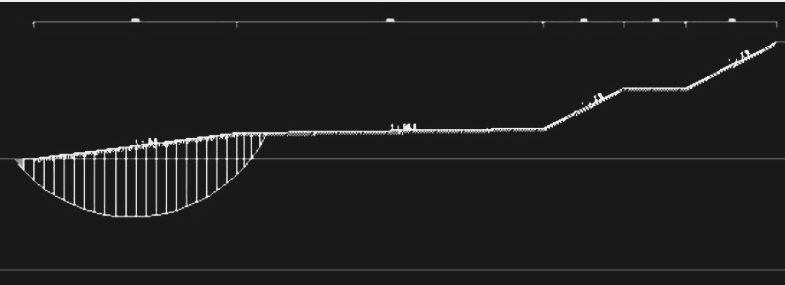
\includegraphics[width=\textwidth]{66.png}
        \caption{斜坡式海堤外坡稳定计算}
        \label{fig:slope_outer}
    \end{minipage}
    \hfill
    \begin{minipage}[b]{0.45\textwidth}
        \centering
        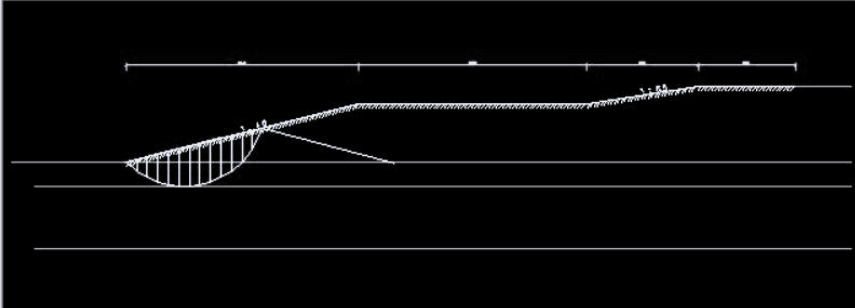
\includegraphics[width=\textwidth]{67.png}
        \caption{斜坡式海堤内坡稳定计算}
        \label{fig:slope_inner}
    \end{minipage}
    \vspace{0.5cm}
    \begin{minipage}[b]{0.45\textwidth}
        \centering
        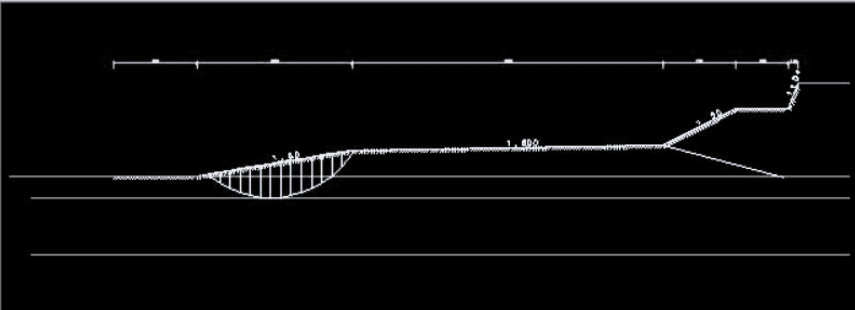
\includegraphics[width=\textwidth]{68.png}
        \caption{混合式海堤外坡稳定计算}
        \label{fig:mixed_outer}
    \end{minipage}
    \hfill
    \begin{minipage}[b]{0.45\textwidth}
        \centering
        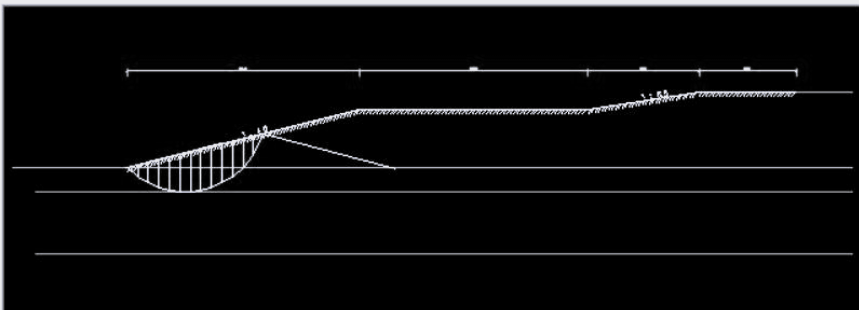
\includegraphics[width=\textwidth]{69.png}
        \caption{混合式海堤内坡稳定计算}
        \label{fig:mixed_inner}
    \end{minipage}
\end{figure}
\newpage
\subsubsection{海堤断面方案比较与选择}
\begin{table}[h]
    \centering
    \caption{斜坡式与混合式海堤断面型式比较表}
    \resizebox{\textwidth}{!}{ % 调整表格宽度以适应页面
    \begin{tabular}{|c|c|c|}
        \hline
        \textbf{断面形式} & \textbf{斜坡式} & \textbf{混合式} \\ \hline
        防浪墙顶高程(m) & 9.5 & 9.0 \\ \hline
        堤顶路面高程(m) & 8.0 & 7.5 \\ \hline
        消浪平台高程(m) & 4.0 & 4.0 \\ \hline
        消浪平台宽度(m) & 6.0 & 5.0 \\ \hline
        临海侧斜坡坡度 & 1:2 & 1:2 \\ \hline
        缓坡镇压平台高程(m) & 0.5-1.0 & 0.5-1.0 \\ \hline
        缓坡镇压平台宽度(m) & 30 & 20 \\ \hline
        护底块石宽度(m) & 20 & 8 \\ \hline
        块石平台边坡 & 1:1.5 & 1:1.5 \\ \hline
        每延米所需工程量(m\textsuperscript{3}) & 680 & 510 \\ \hline
        \textbf{优点} & 
        对沉降适应性好,有成熟的计算理论 & 
        堤顶高程低,爬高小,有成熟的计算理论,工程量最小 \\ \hline
        \textbf{缺点} & 
        波浪爬高大,堤顶高程较高,断面大,投资大 & 
        陆墙施工需等沉降基本稳定后实施,变坡折角处波流混乱,需加强保护 \\ \hline
    \end{tabular}
    }
    \label{tab:comparison_slope_mixed}
\end{table}

\par

综上,采用混合式断面作为造地工程的海堤断面型式。



\begin{figure}[h]
    \centering
    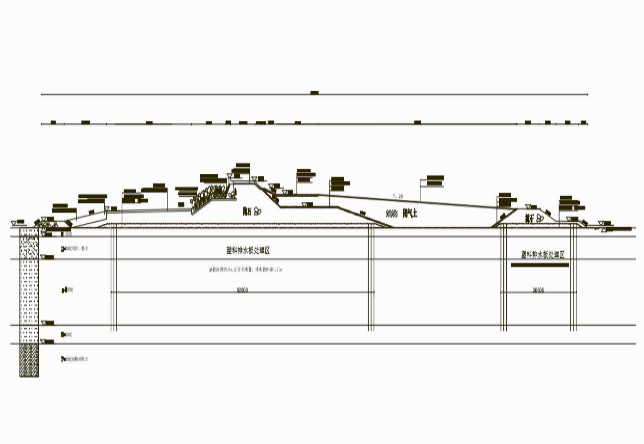
\includegraphics[width=1.0\textwidth]{nb.png}
    \caption{混合式海堤断面图}
    \label{fig:slope_section}
\end{figure}

\newpage
\subsection{堤顶高程}
根据规范来计算确定堤顶高程。白马堤工程为 1 级海堤工程,设计标准为 200 年一遇,混合式海堤堤顶高程计算如
下。

\subsubsection{波浪爬高}
根据《浙江省海塘工程技术规定(上)》,当 $d \geq 2H$,$-1.0 \leq dw/H \leq 1.0$ 时,波浪爬高 $R_{F\%}$ 计算公式为:
\begin{equation}
    R_{F\%} = 1.36 \left( 1.5 H K_z \tanh \frac{2 \pi d}{L} - dw \right) k_y \cdot k_v
\end{equation}

式中:
\begin{itemize}
    \item $d$ —— 堤前水深,单位:$\text{m}$;
    \item $H$ —— 波高,单位:$\text{m}$;
    \item $K_z$ —— 系数,与波浪特性和堤坡有关;
    \item $L$ —— 波长,单位:$\text{m}$;
    \item $dw$ —— 平台高程修正值,单位:$\text{m}$;
    \item $k_y$ —— 修正系数;
    \item $k_v$ —— 风速及堤前水深修正系数。
\end{itemize}

\subsubsection{防浪墙顶高程}
由《海堤工程设计规范》得,防浪墙顶高程用以下公式计算:
\begin{equation}
    Z_p = h_p + R_{F\%} + \Delta h
\end{equation}

式中:
\begin{itemize}
    \item $Z_p$ —— 防浪墙顶高程;
    \item $h_p$ —— 设计频率的高潮位,单位:$\text{m}$;
    \item $R_{F\%}$ —— 波浪爬高,单位:$\text{m}$;
    \item $\Delta h$ —— 安全加高值,单位:$\text{m}$。
\end{itemize}

\subsubsection{堤顶高程}

查阅《海堤工程设计规范》知,堤顶高程应该大于设计高潮位加上一半的累
积频率为 $1\%$的波高值。
\subsubsection{越浪量计算}
由《长波条件下波浪爬高及越浪量研究》得,越浪量计算公式计算如下:



\begin{equation}
    Q = 0.08 \frac{R_s}{H_s} \exp\left(-4 \frac{H_c}{R_s} - 0.9 \frac{P}{H_c}\right) \sqrt{g H_s^3}
\end{equation}

式中:
\begin{itemize}
    \item $Q$ —— 单位时间单位宽海堤上的越浪水量($\text{m}^3/\text{s·m}$);
    \item $H_c$ —— 防浪墙顶至设计高潮位的高度($\text{m}$);
    \item $H_s$ —— 有效波高,对于允许部分越浪的情况,取 $H_{13\%}$($\text{m}$);
    \item $R_s$ —— 有效波浪爬高,对于允许部分越浪的情况,取 $R_{13\%}$($\text{m}$);
    \item $P$ —— 防浪墙高度($\text{m}$),对于堤顶未设置防浪墙的断面 $P = 0$。
\end{itemize}

在有风的情况下,海堤的越浪量计算用以上公式计算结果乘风校正因子 $K'$ 得到。

\begin{equation}
    K' = 1.0 + W_f \left( \frac{H_c}{R} + 0.1 \right) \sin \theta
\end{equation}

式中:
\begin{itemize}
    \item $R$ —— 波浪爬高($\text{m}$);
    \item $H_c$ —— 防浪墙顶至设计高潮位的高度($\text{m}$);
    \item $W_f$ —— 与风速有关,当设计风速 $\geq 23.8\,\text{m/s}$ 时,$W_f = 2.0$;
    \item $\theta$ —— 波浪入射角(度)。
\end{itemize}


\textbf{下乌仙堤A1点:}

\[
R_s = 1.45, \quad H_s = 2.14, \quad H_c = 2.11, \quad P = 0.5
\]

\[
Q' = 0.08 \cdot \frac{R_s}{H_s} \exp\left(-4 \frac{H_c}{R_s} - 0.9 \frac{P}{H_c}\right) \sqrt{9.81 \cdot H_s^3} = 0.00128
\]

\[
K' = 1.0 + 2.0 \left(\frac{H_c}{R_s} + 0.1\right) \cdot 0.46 = 2.431
\]

\[
Q = K' \cdot Q' = 2.431 \cdot 0.00128 = 0.00311
\]

\textbf{下乌仙堤A2点:}

\[
R_s = 1.49, \quad H_s = 2.15, \quad H_c = 2.11, \quad P = 0.5
\]

\[
Q' = 0.08 \cdot \frac{R_s}{H_s} \exp\left(-4 \frac{H_c}{R_s} - 0.9 \frac{P}{H_c}\right) \sqrt{9.81 \cdot H_s^3} = 0.00152
\]

\[
K' = 1.0 + 2.0 \left(\frac{H_c}{R_s} + 0.1\right) \cdot 0.46 = 2.3948
\]

\[
Q = K' \cdot Q' = 2.3948 \cdot 0.00152 = 0.00364
\]

\textbf{下乌仙堤A3点:}

\[
R_s = 1.45, \quad H_s = 2.17, \quad H_c = 2.11, \quad P = 0.5
\]

\[
Q' = 0.08 \cdot \frac{R_s}{H_s} \exp\left(-4 \frac{H_c}{R_s} - 0.9 \frac{P}{H_c}\right) \sqrt{9.81 \cdot H_s^3} = 0.00128
\]

\[
K' = 1.0 + 2.0 \left(\frac{H_c}{R_s} + 0.1\right) \cdot 0.46 = 2.431
\]

\[
Q = K' \cdot Q' = 2.431 \cdot 0.00128 = 0.00311
\]

\textbf{下乌仙堤A4点:}
\[
R_s = 2.36, \quad H_s = 3.18, \quad H_c = 2.11, \quad P = 0.5
\]

\[
Q' = 0.08 \cdot \frac{R_s}{H_s} \cdot \exp\left(-4 \cdot \frac{H_c}{R_s} - 0.9 \cdot \frac{P}{H_c}\right) \cdot \sqrt{9.81 \cdot H_s^3} = 0.00239
\]

\[
K' = 1.0 + 2.0 \cdot \left(\frac{H_c}{R_s} + 0.1\right) \cdot 0.46 = 1.91415
\]

\[
Q = K' \cdot Q' = 1.91415 \cdot 0.00239 = 0.00457
\]

\textbf{下乌仙堤A5点:}
\[
R_s = 2.24, \quad H_s = 3.18, \quad H_c = 2.11, \quad P = 0.5
\]

\[
Q' = 0.08 \cdot \frac{R_s}{H_s} \cdot \exp\left(-4 \cdot \frac{H_c}{R_s} - 0.9 \cdot \frac{P}{H_c}\right) \cdot \sqrt{9.81 \cdot H_s^3} = 0.00232
\]

\[
K' = 1.0 + 2.0 \cdot \left(\frac{H_c}{R_s} + 0.1\right) \cdot 0.46 = 1.9582
\]

\[
Q = K' \cdot Q' = 1.9582 \cdot 0.00232 = 0.00454
\]

计算得,下乌仙堤的最大越浪量位置为A2点,方向为 WSW 向,其最大越浪量为 $0.0364\,\text{m}^3/\text{s·m}$。
白马堤的最大越浪量的位置为白马堤A4点,其有风越浪量最大为 $0.457\,\text{m}^3/\text{s·m}$。
由《海堤工程设计规范》得,堤顶有三面保护的海堤最大允许越浪量为 $0.05\,\text{m}^3/\text{s·m}$,满足设计要求。

\begin{table}[h]
    \centering
    \caption{混合堤设计参数与计算结果}
    \resizebox{0.5\textwidth}{!}{
    \begin{tabular}{|c|c|c|c|}
        \hline
        堤段 & 下乌仙堤A1 & 下乌仙堤A2 & 下乌仙堤A3 \\ \hline
        波向 & $S-SSW$ & $S-SSW$ & $S-SSW$ \\ \hline
        波浪性质 &  风推浪 & 风推浪 & 风推浪 \\ \hline
        重现期 & 200年 & 200年 & 200年 \\\hline
        设计潮位 $h_p$ (m) & 6.89 & 6.89 & 6.89 \\ \hline
        设计风速 $V$ (m/s) & 38.8 & 38.8 & 38.8 \\ \hline
        平均波高 $\bar{H}$ (m) & 1.39 & 1.40 & 1.41 \\ \hline
        平均波周期 $\bar{T}$ (s) & 5.2 & 5.2 & 5.3 \\ \hline
        设计波长 $L$ (m) & 42.6 & 43.0 & 43.4 \\ \hline
        设计波高 $H_{1\%}$ (m) & 3.04 & 3.05 & 3.07 \\ \hline
        设计波高 $H_{13\%}$ (m) & 2.14 & 2.15 & 2.17 \\ \hline
        粒滞系数 $K_\Delta$ & 0.523 & 0.523 & 0.523 \\ \hline
        波向修正系数 $K_\beta$ & 1 & 1 & 1 \\ \hline
        压载系数 $K_y$ & 1 & 1 & 1 \\ \hline
        波浪爬高值 $R_{13\%}$ (m) & 1.45 & 1.49 & 1.45 \\ \hline
        安全加高值 $\Delta h$ (m) & 0.5 & 0.5 & 0.5 \\ \hline
        爬高计算防浪墙顶高程 (m) & 7.55 & 7.93 & 7.20 \\ \hline
        $h_p  + 0.5H_{1\%}$ &8.89&8.90&8.89 \\ \hline
        设计防浪墙顶高程 (m) & 9.0 & 9.0 &9.0 \\ \hline
        有效越浪量 (m\textsuperscript{3}/s·m) & 0.00311 & 0.00364 & 0.00311 \\ \hline
        设计堤顶高程 (m) & 9.0 & 9.5 & 9.0 \\ \hline
    \end{tabular}
    }
    \label{tab:design_parameters}
\end{table}


\begin{table}[h]
    \centering
    \caption{白马堤设计参数与计算结果}
    \begin{tabular}{|c|c|c|}
        \hline
        \textbf{参数} & \textbf{白马堤A4} & \textbf{白马堤A5} \\ \hline
        波向 & $E-ESE$ & $E-ESE$ \\ \hline
        波浪性质 & 浪推浪 & 浪推浪 \\ \hline
        重现期 & 200年 & 200年 \\ \hline
        设计潮位 $h_p$ (m) & 6.89 & 6.89 \\ \hline
        设计风速 $V$ (m/s) & 38.8 & 38.8 \\ \hline
        平均波高 $\bar{H}$ (m) & 2.10 & 2.10 \\ \hline
        平均波周期 $\bar{T}$ (s) & 13.4 & 13.4 \\ \hline
        设计波长 $L$ (m) & 131.4 & 131.4 \\ \hline
        设计波高 $H_{1\%}$ (m) & 4.40 & 4.40 \\ \hline
        设计波高 $H_{13\%}$ (m) & 3.18 & 3.18 \\ \hline
        粒滞系数 $K_\Delta$ & 0.523 & 0.523 \\ \hline
        波向修正系数 $K_\beta$ & 1 & 1 \\ \hline
        压载系数 $K_y$ & 1 & 1 \\ \hline
        波浪爬高值 $R_{13\%}$ (m) & 2.36 & 2.24 \\ \hline
        安全加高值 $\Delta h$ (m) & 0.5 & 0.5 \\ \hline
        爬高计算防浪墙顶高程 (m) & 9.75 & 9.75 \\ \hline
        $h_p + 0.5H_{1\%}$ & 9.09 & 9.09 \\ \hline
        设计防浪墙顶高程 (m) & 9.0 & 9.0 \\ \hline
        有效越浪量 (m\textsuperscript{3}/s·m) & 0.00457 & 0.00454 \\ \hline
        设计堤顶高程 (m) & 9.0 & 9.0 \\ \hline
    \end{tabular}
    \label{tab:white_horse_dike_parameters}
\end{table}
\newpage

\subsection{海堤基础处理}
洞头区的主要地基为 软土地基,主要由淤泥、淤泥质粘土、粉质粘土等组成。这些地基土层具有高含水量、低强度和高压缩性,容易引起较大的地基沉降,因此在工程设计中需要进行地基加固和沉降控制处理。
采用塑料排水插板法进行地基处理,地基插入深度为 25\,\text{m},$b=100\,\text{mm}$,$\delta=5.0\,\text{mm}$。  
正方形排列,排水板间距取为 1.20\,\text{m}。

由《海堤工程设计规范》得,塑料排水板的当量换算直径计算公式如下:
\begin{equation}
    d_p = \alpha \frac{2(b + \delta)}{\pi}
\end{equation}

式中:
\begin{itemize}
    \item $d_p$ —— 塑料排水板当量换算直径,单位:$\text{mm}$;
    \item $b$ —— 塑料排水板宽度,单位:$\text{mm}$;
    \item $\delta$ —— 塑料排水板厚度,单位:$\text{mm}$;
    \item $\alpha$ —— 换算系数,可取 $\alpha = 0.75$。
\end{itemize}
由《海堤工程设计规范》得,塑料排水板的当量换算直径计算公式如下:
\begin{equation}
    d_p = \alpha \frac{2(b + \delta)}{\pi}
\end{equation}

代入数据:
\[
    d_p = 0.75 \times \frac{2 \times (100 + 4.0)}{\pi} = 49.656\,\text{mm}
\]

有效排水直径计算公式如下:
\[
    d_e = 1.131
\]

式中:
\begin{itemize}
    \item $d_e$ —— 塑料排水板有效排水直径,单位:$\text{mm}$;
    \item $l$ —— 塑料排水板正方形排列的间距,为 $1200\,\text{mm}$。
\end{itemize}

代入数据:
\[
    d_e = 1.13 \times 1200 = 135.6\,\text{mm}
\]



塑料排水法可以加快地基的排水固结,从而增加地基的承载力,较小地基的沉降量。此外,该技术较为成熟,且通过塑料排水法进行地基处理有着较长的周期,还需要海堤的自重较大才可以确保地基处理的成功。塑料排水法还具有成本低、污染少等特点,较为适合本工程。

查《塑料排水板施工规范》,综合考虑地基条件、经济成本与环境保护等条件,最终选取 B 型塑料排水板进行地基处理。海堤地基土主要为淤泥,故需对海堤石段以下地基经行处理。淤泥厚度达 23 米以上,选取 B 型塑料排水板,恰好可以对大部分淤泥进行地基处理。

B 型塑料排水板采用正方形排列,间距 1.2\,\text{m}。在采用塑料排水板法的处理区沿面上共铺设有两层土工织布,均为 50\,\text{kN/m} 的分土工织布。两层土工布中间设厚 1\,\text{m} 的碎石垫层,在碎石垫层上插设塑料排水板。

进行地基处理后,下乌仙堤和白马堤的整体稳定安全系数均为 1.30 以上。

\subsection{海堤闭气处理}

闭气处理方案设计如下:
\begin{itemize}
    \item 顶高程:$9.0\,\text{m}$;
    \item 顶部宽度:$1.0\,\text{m}$;
    \item 顶部与坡顶连接坡度:$1:1.5$;
    \item 以海堤 III0 层淤泥作为闭气土方;
    \item 平台下与海堤涂面相交段坡度:$1:2$;
    \item 闭气土层上层护面铺设混凝土路面;
    \item 二级平台以坡度 $1:20$ 的边坡与子堤相连;
    \item 子堤设两级平台,平台高程分别为 $1.00\,\text{m}$ 和 $-1.00\,\text{m}$;
    \item 平台宽度为 $8\,\text{m}$。
\end{itemize}



\begin{table}[h]
    \centering
    \caption{下乌仙堤与白马堤设计参数对比表(上)}
    \begin{tabular}{|c|c|c|}
        \hline
        \textbf{参数} & \textbf{下乌仙堤} & \textbf{白马堤} \\ \hline
        内设平台高程 (m) & 1.50 & 1.50 \\ \hline
        平台宽度 (m) & 20 & 20 \\ \hline
        闭气土顶高程 (m) & 6.0 & 6.0 \\ \hline
        闭气土表面材料 & 三维土工垫 & 三维土工垫 \\ \hline
        抛石子堤一级平台高程 (m) & 1.00 & 1.00 \\ \hline
        抛石子堤二级平台高程 (m) & -1.00 & -1.00 \\ \hline
    \end{tabular}
    \label{tab:west_south_dike_comparison_part1}
\end{table}

\begin{table}[h]
    \centering
    \caption{下乌仙堤与白马堤设计参数对比表(下)}
    \begin{tabular}{|c|c|c|}
        \hline
        \textbf{参数} & \textbf{下乌仙堤} & \textbf{白马堤} \\ \hline
        平台宽度 (m) & 8.0 & 8.0 \\ \hline
        堤顶高程 (m) & 7.75 & 8.00 \\ \hline
        堤顶宽度 (m) & 8.50 & 8.50 \\ \hline
        堤顶建筑材料 & 20cm 厚自然级配石渣和 &20cm 厚自然级配石渣和\\ 
        & 30cm 厚度的 C20 混凝土路面 &  30cm 厚度的 C20 混凝土路面\\ \hline
        防浪胸墙形式 & L 型 & L 型 \\ \hline
    \end{tabular}
    \label{tab:west_south_dike_comparison_part2}
\end{table}



\subsection{护坡坡脚处理}
\subsection{块石稳定重量计算}

下乌仙堤的临海侧缓坡压压平台与护底块石平台相连接的 1:6 边坡采用大块石两层铺设。
白马堤的消浪平台和护底块石采用扭王字块的布置方式,缓坡压压平台与护底块体平台相连接的 1:4 边坡采用大块石两层铺设。

\subsubsection{块石稳定重量计算}

对于采用规则块石上升型块体或变坡分递的块石,块石的稳定重量 $Q$(海堤工程设计规范)计算公式如下:

\begin{equation}
Q = 0.1 \frac{\gamma_b H^3}{K_D \left( \frac{\gamma_b}{\gamma} - 1 \right)^3 m} 
\end{equation}

式中:
\begin{itemize}
    \item $Q$ —— 块石稳定重量;
    \item $\gamma_b$ —— 块石重度,取当地石料的建议重度 $23.0\,\text{kN/m}^3$;
    \item $\gamma$ —— 水重度,$9.81\,\text{kN/m}^3$;
    \item $H$ —— 设计波高,单位:$\text{m}$;
    \item $K_D$ —— 稳定系数,按规范表 J.0.6-1 取值,为 $21$;
    \item $m$ —— 斜坡坡比。
\end{itemize}

\subsubsection{计算示例}

已知参数:
\begin{itemize}
    \item $\gamma_b = 23.0\,\text{kN/m}^3$;
    \item $\gamma = 9.81\,\text{kN/m}^3$;
    \item $H = 2.03\,\text{m}$;
    \item $K_D = 21$;
    \item $m = 2.1$。
\end{itemize}

代入公式:
\[
Q = 0.1 \cdot \frac{23.0 \cdot 2.03^3}{21 \cdot \left( \frac{23.0}{9.81} - 1 \right)^3 \cdot 2.1}
\]

计算得:
\[
Q = 0.1 \cdot \frac{23.0 \cdot 8.36}{21 \cdot \left( 2.34 - 1 \right)^3 \cdot 2.1} = 0.1 \cdot \frac{192.28}{21 \cdot 1.34^3 \cdot 2.1} = 0.1 \cdot \frac{192.28}{21 \cdot 2.41 \cdot 2.1} = 0.1 \cdot \frac{192.28}{106.61} \approx 1.80\,\text{t}
\]

最终结果:
\[
Q \approx 1.80\,\text{t}
\]
\subsection{海堤沉降量计算}


\begin{equation}
    S = m \sum_{i=1}^n \frac{e_{1i} - e_{2i}}{1 + e_{1i}} h_i
    \label{eq:settlement}
\end{equation}

式中:
\begin{itemize}
    \item $S$ —— 最终沉降量,单位:$\text{mm}$;
    \item $n$ —— 计算分层的土层数;
    \item $e_{1i}$ —— 第 $i$ 土层的初始孔隙比;
    \item $e_{2i}$ —— 第 $i$ 土层在平均自重应力和平均附加应力作用下的孔隙比;
    \item $h_i$ —— 第 $i$ 土层的厚度,单位:$\text{mm}$;
    \item $m$ —— 沉降系数,对软土地基 $m = 1.3 \sim 1.6$,考虑本工程的土层主要为淤泥,取 $1.60$。
\end{itemize}

\subsection{海堤的防渗设计}
为保持海堤渗透稳定性,应满足以下公式:
\begin{equation}
    L \geq C \Delta h; \quad y \geq k \frac{\gamma \Delta H}{\gamma_b}
\end{equation}

式中:
\begin{itemize}
    \item $L$ —— 海堤的宽度,单位:$\text{m}$;
    \item $C$ —— 渗径系数;
    \item $\Delta h$ —— 海堤两次的最高水头差,单位:$\text{m}$;
    \item $y$ —— 验算点到土体表面的最短距离,单位:$\text{m}$;
    \item $k$ —— 安全系数,取为 $1.20$;
    \item $\gamma$ —— 水的重度,单位:$\text{kN/m}^3$;
    \item $\gamma_b$ —— 土的重度,单位:$\text{kN/m}^3$;
    \item $\Delta H$ —— 作用水头,单位:$\text{m}$。
\end{itemize}


\textbf{下乌仙堤:}

\[
L = 188.05\,\text{m}, \quad C = 8.0, \quad \Delta h = 5.94\,\text{m}
\]

\[
y = 3.11\,\text{m}, \quad \Delta H = 4.94\,\text{m}, \quad \gamma = 9.81\,\text{kN/m}^3, \quad \gamma_b = 22.0\,\text{kN/m}^3
\]

\[
C \times \Delta h = 8.0 \times 5.94 = 47.52\,\text{m}, \quad k \frac{\gamma \Delta H}{\gamma_b} = 1.20 \times \frac{9.81 \times 4.94}{22.0} = 2.64\,\text{m}
\]

因此下乌仙堤满足防渗要求。

\textbf{白马堤:}

\[
L = 184.03\,\text{m}, \quad C = 8.0, \quad \Delta h = 5.22\,\text{m}
\]

\[
y = 2.77\,\text{m}, \quad \Delta H = 4.22\,\text{m}, \quad \gamma = 9.81\,\text{kN/m}^3, \quad \gamma_b = 22.0\,\text{kN/m}^3
\]

\[
C \times \Delta h = 8.0 \times 5.22 = 41.76\,\text{m}, \quad k \frac{\gamma \Delta H}{\gamma_b} = 1.20 \times \frac{9.81 \times 4.22}{22.0} = 2.26\,\text{m}
\]

因此白马堤满足防渗要求。


\subsection{海堤挡墙的稳定性计算}

\subsubsection{挡墙及防浪胸墙的设计}
在海堤临海侧消浪平台上设置挡墙,作为组合式海堤的上部结构。
东堤和北堤的挡墙如下图所示,挡墙的外坡的坡度为1:0.4,
内坡的坡度为1:0.2。
挡墙的主体采用灌砂块石混凝土,表面采用40cm的条石护面。
在挡墙上部设置防浪墙,防浪墙采用钢筋混凝土构成,将防浪墙与挡墙浇筑成整体。
南堤的挡墙的净高为4.00m,底部宽度为3.00m,防浪墙的顶宽度为0.50m。
西堤的挡墙的净高为4.50m,底部宽度为3.75m。
北堤防浪墙的顶宽度为0.75m。
防浪墙的底部埋深为0.50m。
\subsubsection{挡墙的作用力计算}
\begin{itemize}
    \item 挡墙的自重 $W$;
\end{itemize}
\begin{itemize}
    \item 墙前波浪作用力 $P$;
\end{itemize}
\begin{itemize}
    \item 墙后土压力 $P_1$;
\end{itemize}

挡墙后的主动土压力计算:

\begin{equation}
K_a = \tan^2 \left( 45^\circ - \frac{\varphi}{2} \right) 
\end{equation}
式中:
\begin{itemize}
    \item $K_a$ —— 朗肯理论中的主动土压力系数;
    \item $\varphi$ —— 土的破碎角,取 $\varphi = 40^\circ$。
\end{itemize}

代入数据:
\[
K_a = \tan^2 \left( 45^\circ - \frac{40^\circ}{2} \right) = 0.3072
\]

\[
K_a = \frac{\cos^2 (\varphi - \epsilon)}{\cos^2 (\varphi + \varphi_0)} \left[ 1 + \frac{\sin (\epsilon + \alpha) \sin (\varphi - \alpha)}{\cos (\epsilon + \alpha) \cos (\varphi - \alpha)} \right]
\]

式中:
\begin{itemize}
    \item $K_a$ —— 库仑理论中的主动土压力系数;
    \item $\varphi$ —— 土的破碎角,取 $\varphi = 40^\circ$;
    \item $\varphi_0$ —— 墙背与填土的摩擦角,取 $\varphi_0 = \varphi / 3$;
    \item $\alpha$ —— 墙土表面与水平面的夹角,取 $\alpha = 0^\circ$;
    \item $\epsilon$ —— 墙土表面与水平面的夹角,$\epsilon = 11.31^\circ$。
\end{itemize}

\[
K_a = \frac{\cos^2 \left( 40^\circ - 11.31^\circ \right)}{\cos^2 \left( 11.31^\circ \cos \left( 11.31^\circ + 13.3^\circ \right) \right)} 
\left[ 
1 + \sqrt{\frac{\sin \left( 40^\circ + 11^\circ \right) \sin \left( 40^\circ - 0^\circ \right)}{\cos \left( 11.31^\circ + 13.3^\circ \right) \cos \left( 11.31^\circ - 0^\circ \right)}}
\right]
\]

\[
K_a = 0.1203
\]

利用式 (3.2.27) 计算得到,主动土压力系数 $K_{a1} = 0.3072$。利用式 (3.2.28) 计算得到,主动土压力系数 $K_{a2} = 0.1203$。

因此,挡墙后的主动土压力可以计算如下:

\[
E_{a1} = \frac{1}{2} \gamma_1 H_1^2 K_{a1} 
\]

\[
E_{a2} = \gamma_1 H_1 H_2 K_{a2} 
\]

\[
E_{a3} = \frac{1}{2} \gamma_2 H_2^2 K_{a2} 
\]

\[
E_a = E_{a1} + E_{a2} + E_{a3} 
\]

由以上公式计算西堤挡土墙的墙后主动土压力,$H_1 = 0.50\,\text{m}$,$H_2 = 4.35\,\text{m}$。

北堤挡土墙:$H_1 = 0.50\,\text{m}$,$H_2 = 3.50\,\text{m}$。计算得到西堤挡土墙主动土压力和南堤挡土墙主动土压力分别为 $26.8195\,\text{kN}$ 和 $18.61993\,\text{kN}$。

\[
E_{a1} = \frac{1}{2} \times 23.0 \times 0.50^2 \times 0.3072 = 0.8832\,\text{kN}
\]

\[
E_{a2} = 23.0 \times 0.50 \times 4.35 \times 0.1203 = 6.0181\,\text{kN}
\]

\[
E_{a3} = \frac{1}{2} \times 17.5 \times 4.35^2 \times 0.1203 = 19.9183\,\text{kN}
\]

\[
E_a = 0.8832 + 6.0181 + 19.9183 = 26.8195\,\text{kN}
\]


挡墙后的被动土压力计算公式如下:

\begin{equation}
K_a = \tan^2 \left( 45^\circ + \frac{\varphi}{2} \right) 
\end{equation}
式中:
\begin{itemize}
    \item $K_p$ —— 朗肯理论中的被动土压力系数;
    \item $\varphi$ —— 土的破碎角,取 $\varphi = 40^\circ$。
\end{itemize}

代入数据:
\[
K_p = \tan^2 \left( 45^\circ + \frac{40^\circ}{2} \right) = 3.2544
\]

\[
K_p = \frac{\cos^2 (\varphi + \epsilon)}{\cos^2 (\epsilon - \varphi_0)} 
\left[ 
1 - \frac{\sin (\epsilon + \varphi_0) \sin (\varphi + \alpha)}{\cos (\epsilon + \varphi_0) \cos (\varphi - \alpha)}
\right] 
\]

式中:
\begin{itemize}
    \item $K_p$ —— 库仑理论中的被动土压力系数;
    \item $\varphi$ —— 土的破碎角,取 $\varphi = 40^\circ$;
    \item $\varphi_0$ —— 墙背与填土的摩擦角,取 $\varphi_0 = \varphi / 3$;
    \item $\alpha$ —— 墙土表面与水平面的夹角,取 $\alpha = 0^\circ$;
    \item $\epsilon$ —— 墙土表面与水平面的夹角,$\epsilon = 11.31^\circ$。
\end{itemize}

代入数据:
\[
K_p = \frac{\cos^2 \left( 40^\circ + 11.31^\circ \right)}{\cos^2 \left( 11.31^\circ - 13.3^\circ \right)} 
\left[ 
1 - \frac{\sin \left( 40^\circ + 11^\circ \right) \sin \left( 40^\circ - 0^\circ \right)}{\cos \left( 11.31^\circ + 13.3^\circ \right) \cos \left( 11.31^\circ - 0^\circ \right)}
\right]
\]

计算得:
\[
K_p = 4.0423
\]

计算得到,被动土压力系数 $K_{p1} = 3.2544$。 计算得到,主动土压力系数 $K_{p2} = 1.0423$。

因此,挡墙后的主动土压力可以计算如下:

\[
E_{p1} = \frac{1}{2} \gamma_1 H_1^2 K_{p1} 
\]

\[
E_{p2} = \gamma_1 H_1 H_2 K_{p2} 
\]

\[
E_{p3} = \frac{1}{2} \gamma_2 H_2^2 K_{p2} 
\]

\[
E_p = E_{p1} + E_{p2} + E_{p3} 
\]

根据以上公式计算西堤挡土墙后的被动土压力:$H_1 = 0.50\,\text{m}$,$H_2 = 4.35\,\text{m}$。

北堤挡土墙:$H_1 = 0.50\,\text{m}$,$H_2 = 3.50\,\text{m}$。计算得到西堤挡土墙被动土压力和南堤挡土墙被动土压力分别为 $243.073\,\text{kN}$ 和 $163.005\,\text{kN}$。

\[
E_{p1} = \frac{1}{2} \times 23.0 \times 0.50^2 \times 3.2544 = 9.3564\,\text{kN}
\]

\[
E_{p2} = 23.0 \times 0.50 \times 4.35 \times 1.0423 = 52.1412\,\text{kN}
\]

\[
E_{p3} = \frac{1}{2} \times 17.5 \times 4.35^2 \times 1.0423 = 172.5756\,\text{kN}
\]

\[
E_p = 9.3564 + 52.1412 + 172.5756 = 243.073\,\text{kN}
\]
\subsubsection{挡墙的滑动稳定性计算}

根据《浙江省海塘工程技术规定下册》,挡墙的滑动稳定性应满足以下条件:

\[
K_c > 1.15
\]

其中,抗滑稳定安全系数 $K_c$ 的计算公式为:

\begin{equation}
    K_c = \frac{f \cdot \sum W}{\sum P}
\end{equation}

式中:
\begin{itemize}
    \item $K_c$ —— 抗滑稳定安全系数;
    \item $\sum P$ —— 作用于墙上的全部水平力的总和(单位:$\text{kN}$);
    \item $\sum W$ —— 作用于墙上的全部垂直力的总和(单位:$\text{kN}$);
    \item $f$ —— 挡墙底部与墙基之间的摩擦系数,取值为 $0.6$。
\end{itemize}
\subsubsection{挡墙的滑动稳定性计算}

(1) 挡墙向海侧的滑动稳定性计算

西堤挡墙的向海侧滑动稳定性计算如下:

\[
\sum P = E_a = 26.8195\,\text{kN}
\]

\[
\sum W = G = 368.863\,\text{kN}
\]

\[
K_c = \frac{0.60 \times 368.863}{26.8195} = 8.252
\]

满足稳定性要求。

南堤挡墙的向海侧滑动稳定性计算如下:

\[
\sum P = E_a = 18.6199\,\text{kN}
\]

\[
\sum W = G = 231.075\,\text{kN}
\]

\[
K_c = \frac{0.60 \times 231.075}{18.6199} = 7.446
\]

满足稳定性要求。

(2) 挡墙向陆侧的滑动稳定性计算

西堤挡墙的向陆侧滑动稳定性计算如下:

\[
\sum P = P - E_p = 240.0801 - 234.073 = 6.0071\,\text{kN}
\]

\[
\sum W = G - P_u = 368.863 - 167.7766 = 201.0862\,\text{kN}
\]

\[
K_c = \frac{0.60 \times 201.0862}{6.0071} = 20.085
\]

满足稳定性要求。

南堤挡墙的向陆侧滑动稳定性计算如下:

\[
\sum P = P - E_p = 181.1604 - 163.0305 = 18.1299\,\text{kN}
\]

\[
\sum W = G - P_u = 231.075 - 97.0541 = 134.0209\,\text{kN}
\]

\[
K_c = \frac{0.60 \times 134.0209}{18.1299} = 4.435
\]

满足稳定性要求。
\subsubsection{挡墙的倾覆稳定性计算}
根据《浙江省海塘工程技术规定下册》,防护墙的抗倾覆稳定安全系数可以按下式计算,$K_0$ 应大于 $1.50$。

\begin{equation}
K_0 = \frac{\sum M_v}{\sum M_H}
\end{equation}



式中:
\begin{itemize}
    \item $K_0$ —— 抗倾覆稳定安全系数;
    \item $\sum M_v$ —— 抗倾覆力矩(单位:$\text{kN·m}$);
    \item $\sum M_H$ —— 倾覆力矩(单位:$\text{kN·m}$)。
\end{itemize}
(1) 挡墙向海侧倾覆稳定性计算

由于低潮位时,挡墙受到的波压力和浮托力很小。因此挡墙的稳定力矩完全由墙后的主动土压力绕前趾(A)点产生的。

西堤挡墙的向海侧倾覆稳定性计算如下:

\[
\sum M_v = 909.760\,\text{kN·m}
\]

\[
\sum M_H = 45.960\,\text{kN·m}
\]

\[
K_0 = \frac{\sum M_v}{\sum M_H} = \frac{909.760}{45.960} = 19.795
\]

满足稳定性要求。

南堤挡墙的向海侧倾覆稳定性计算如下:

\[
\sum M_v = 452.647\,\text{kN·m}
\]

\[
\sum M_H = 16.503\,\text{kN·m}
\]

\[
K_0 = \frac{\sum M_v}{\sum M_H} = \frac{452.647}{16.503} = 16.503
\]

满足稳定性要求。


\subsubsection{挡墙的向陆侧倾覆稳定性计算}

挡墙的向陆侧倾覆稳定性计算示意如下:

\subsubsection{挡墙抗倾、抗滑稳定计算成果表}
下乌仙堤挡墙和白马堤挡墙抗倾覆、抗滑稳定计算成果见表,经计算挡墙的稳定性满足规范要求。

\begin{table}[h]
    \centering
    \caption{挡墙抗倾、抗滑稳定计算成果表}
    \begin{tabular}{|c|c|c|c|c|}
        \hline
        \textbf{计算位置} & \textbf{计算项目} & \textbf{向海侧} & \textbf{向陆侧} & \textbf{规范允许值} \\ \hline
        下乌仙堤 & 抗倾覆稳定 & 19.80 & 1.87 & 1.60 \\ \hline
        下乌仙堤 & 抗滑稳定 & 8.25 & 20.09 & 1.15 \\ \hline
        白马堤 & 抗倾覆稳定 & 16.50 & 1.93 & 1.60 \\ \hline
        白马堤 & 抗滑稳定 & 7.75 & 4.44 & 1.15 \\ \hline
    \end{tabular}
    \label{tab:stability_results}
\end{table}
\section{水闸设计}
\subsection{水闸的平面布置}
\subsection{水闸结构的布置形式}

由于本工程需要布置数量较多的水闸,供可选择的水闸方案也较多。选择 闸为典型闸作为本阶段的设计分析和比较。

\begin{table}[h]
    \centering
    \caption{水闸结构方案}
    \begin{tabular}{|c|c|c|c|}
        \hline
        \textbf{项目} & \textbf{方案一} & \textbf{方案二} & \textbf{方案三} \\ \hline
        溢水孔 & 4 孔 $\times$ 10m & 5 孔 $\times$ 16m & 5 孔 $\times$ 16m \\ \hline
        闸门型式 & 框架式钢闸门 & 弧形钢闸门 & 框架式钢闸门 \\ \hline
        布置方向 & 顺水流方向 & 顺水流方向 & 顺水流方向 \\ \hline
        船闸长度(m) & 22.0 & 52.0 & 28.0 \\ \hline
        闸底板厚度(m) & 1.5 & 1.5 & 1.5 \\ \hline
        闸墩厚度(m) & 2.5 & 4.0 & 2.0 \\ \hline
        变形缝间距(m) & 20 & 20 & 19 \\ \hline
        总宽度(m) & 101 & 100 & 95 \\ \hline
    \end{tabular}
    \label{tab:sluice_structure_options}
\end{table}

由投资金额、当地地基质量,以及对波浪的承载能力的综合考虑,选择方案一作为本工程水闸施工方案。




\subsection{结构设计}
在水闸上游设置消力池,下游设置由砾砾块石浆砌而成的海漫,闸底设置有 C80PHC 预应力管桩。

\begin{table}[h]
    \centering
    \caption{水闸结构设计}
    \begin{tabular}{|c|c|}
        \hline
        \textbf{项目} & \textbf{参数值} \\ \hline
        上游消力池底高程(m) & -2.7 \\ \hline
        上游消力池深度(m) & 0.7 \\ \hline
        上游消力池长度(m) & 24.0 \\ \hline
        下游消力池水深(m) & 1.50 \\ \hline
        第一级消力池长度(m) & 26.0 \\ \hline
        第二级消力池长度(m) & 27.0 \\ \hline
        下游消力池底高程(m) & -3.50 \\ \hline
    \end{tabular}
    \label{tab:sluice_structure_design}
\end{table}
\section{排水渠设计}
依据防洪防潮、新机场建设的需要,拟定排水渠的布置方案。在围区内布置 2 条排水渠,将造地区域分 3 个围区。排水渠两侧护岸采用隔堤式结构设计,两条隔堤采用全抛石断面的结构型式。

\subsubsection{堤顶高程的确定}
排水渠两侧护岸按隔堤堤顶高程计算,选取 50 年一遇为标准,增加 0.5m 安全超高,拟采用顶部高程为 5.50m。
\newpage
\subsubsection{排水渠护岸断面结构}
\begin{table}[h]
    \centering
    \caption{排水渠断面结构设计}
    \begin{tabular}{|c|c|}
        \hline
        \textbf{项目} & \textbf{参数值} \\ \hline
        堤顶高程(m) & 5.50 \\ \hline
        堤顶材料 & 自然石渣和 C20 松护面的宽度为 8.00m 的道路 \\ \hline
        一级平台高程(m) & 3.50 \\ \hline
        一级平台宽度(m) & 3.50 \\ \hline
        二级平台高程(m) & 0.50 \\ \hline
        二级平台宽度(m) & 2.50 \\ \hline
        两级平台之间的坡度 & 1:1.5 \\ \hline
        涂面与二级平台之间坡度 & 1:2 \\ \hline
    \end{tabular}
    \label{tab:drainage_channel_structure}
\end{table}

\begin{figure}[h]
    \centering
    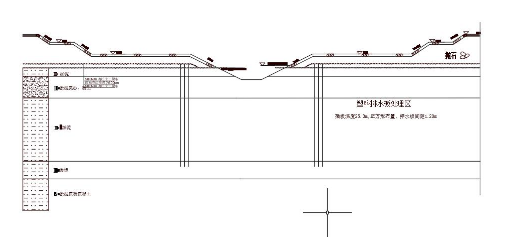
\includegraphics[width=0.8\textwidth]{666.png}
    \caption{排水渠护岸断面结构示意图}
    \label{fig:drainage_channel_structure}
\end{figure}

\section{堵口设计}
\subsection{设计标准}
本工程龙口度汛采用 20 年一遇标准,堵口度汛 10 年一遇高潮位和其典型潮
型。
\subsection{龙口合龙时间选择}
选择合适的龙口合龙时间,是顺利实现龙口合龙的重要因素。黄岙围涂工程白马堤
位于我国东南沿海的温州市,农历 10 月小潮期高潮潮位较低、潮差较小,选择该时段
进行合龙,可以有效降低截流堤的堤顶高程,从而在一定程度上减少堵口工程量。



\subsection{龙口合龙的条件}

\begin{enumerate}
    \item 非龙口段海堤堤身全线石堤断面已达设计高程,土方闭气在高程 $6.0\,\text{m}$ 以下按设计断面完成;
    \item 机械设备、石料均已准备就绪,可以达到龙口合龙施工强度的要求,龙口合龙技术措施均已交底;
    \item 排水闸可以正常启闭,纳潮闸已接近完工;
    \item 龙口合龙申请报告已经取得主管部门批准。
\end{enumerate}

\subsection{龙口位置的选择}
龙口应选址在地质条件较好的区域,以便减少龙口冲刷、增强堤身稳定;考虑到削
减围区内外港的水头差,增强截流堤的稳定性,龙口布置的位置应方便围区内外港的水
量交换;此外,考虑到堤头的稳定性问题,龙口位置应尽量选择在涂面较为低洼的地段,
这样口门处可以保持一定的水深,能起到水垫消能的功效。
\subsection{龙口尺寸的预估}


龙口口门的具体尺寸由水力计算后确定,这里先根据一种近似方法进行预估,以便进行龙口水力计算时对龙口的宽度范围有一个大致的判断。龙口口门宽度估算公式如下所示:

\begin{equation}
    B = \frac{V}{v \cdot t \cdot h} 
\end{equation}

式中:
\begin{itemize}
    \item $B$ —— 龙口口门宽度($\text{m}$);
    \item $V$ —— 龙口吞吐量($\text{m}^3$);
    \item $v$ —— 龙口吞吐平均流速($\text{m/s}$);
    \item $t$ —— 涨潮、退潮历时中的较小者($\text{s}$);
    \item $h$ —— 龙口口门过水断面平均高度($\text{m}$)。
\end{itemize}

\[
B = \frac{5939881}{0.8 \times 3600 \times 5 \times 2.01} = 205.22\,\text{m}
\]

故预估口门宽度为 $200\,\text{m}$,底槽高程为 $2\,\text{m}$。


\subsection{龙口水力计算}
\subsubsection{龙口合龙设计潮位及设计潮型的选择}

堵口设计潮型定为 10 年一遇非汛期最高潮位典型潮型,设计潮位及过程线如下所
示:

\begin{table}[h]
    \centering
    \caption{表 9.1 龙口水力计算设计潮位表}
    \begin{tabular}{cccc}
        \toprule
        \textbf{时段($\Delta t = 3600\,\text{s}$)} & \textbf{潮位(m)} & \textbf{时段($\Delta t = 3600\,\text{s}$)} & \textbf{潮位(m)} \\ 
        \midrule
        1  & 2.06 & 13 & 1.61 \\ 
        2  & 3.93 & 14 & 3.39 \\ 
        3  & 5.08 & 15 & 4.89 \\ 
        4  & 5.40 & 16 & 5.34 \\ 
        5  & 4.95 & 17 & 4.68 \\ 
        6  & 3.89 & 18 & 3.45 \\ 
        7  & 2.63 & 19 & 2.22 \\ 
        8  & 1.49 & 20 & 1.10 \\ 
        9  & 0.63 & 21 & 0.29 \\ 
        10 & -0.05 & 22 & -0.32 \\ 
        11 & -0.51 & 23 & -0.73 \\ 
        12 & 0.02 & 24 & 0.13 \\ 
        \bottomrule
    \end{tabular}
    \label{tab:dragon_port_tide_table}
\end{table}

\begin{figure}[h]
    \centering
    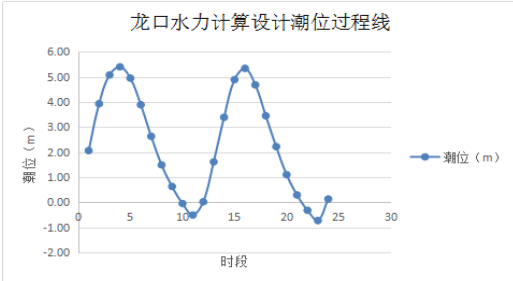
\includegraphics[width=0.8\textwidth]{figurenb.png}
    \caption{龙口水力计算设计潮位过程线}
    \label{fig:dragon_port_tide_process}
\end{figure}

\subsection{围区库容曲线}

围区库容曲线表示围涂区域内水位与该围区库容之间的关系,纵坐标为围区库容,
横坐标为内水位值,具体如下所示:

\begin{table}[h]
    \centering
    \caption{围区库容曲线}
    \begin{tabular}{|c|c|}
        \hline
        \textbf{水位 (m)} & \textbf{库容 (万立方米)} \\ \hline
        -0.50 & 0 \\ \hline
        0.00 & 23.46 \\ \hline
        0.50 & 78.12 \\ \hline
        1.00 & 116.37 \\ \hline
        1.50 & 274.47 \\ \hline
        2.00 & 402.30 \\ \hline
        2.50 & 540.03 \\ \hline
        3.00 & 824.03 \\ \hline
        3.50 & 1104.0 \\ \hline
        4.00 & 1392.0 \\ \hline
    \end{tabular}
    \label{tab:storage_capacity_curve}
\end{table}


\begin{figure}
    \centering
    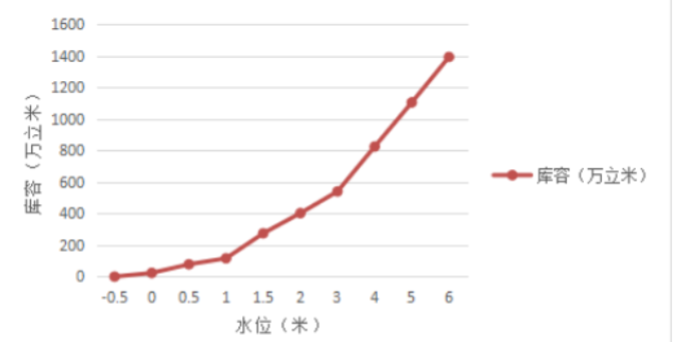
\includegraphics[width=0.8\textwidth]{figurenb2.png}
    \caption{围区库容曲线}
    \label{fig:storage_capacity_curve}
\end{figure}


\newpage
\subsection{计算原理}
根据《堤防工程设计规范》(GB/T51015-2014),利用水量平衡的方法,由围区外设计潮位过程线推求围区内水位过程线,并进而推求涨落潮过程中各项龙口水力要素指标。

根据围区进出水量平衡原理,按如下公式进行计算:

\begin{equation}
    \left[ \bar{Q}_{\text{内}} \pm \left( \bar{Q}_{\text{闸}} + \bar{Q}_{\text{溢}} + \bar{Q}_{\text{渗}} \right) \right] \cdot \Delta t = V_2 - V_1 
\end{equation}

式中:
\begin{itemize}
    \item $\bar{Q}_{\text{内}}$ —— 计算时段内陆域来水平均流量($\text{m}^3/\text{s}$);
    \item $\bar{Q}_{\text{闸}}$ —— 计算时段内水闸泄洪平均流量($\text{m}^3/\text{s}$);
    \item $\bar{Q}_{\text{溢}}$ —— 计算时段内龙口溢流平均流量($\text{m}^3/\text{s}$);
    \item $\bar{Q}_{\text{渗}}$ —— 计算时段内堆石体渗透平均流量($\text{m}^3/\text{s}$);
    \item $\Delta t$ —— 计算时段,这里取 $3600\,\text{s}$;
    \item $V_2$ —— 计算时段末围区库容($\text{m}^3$);
    \item $V_1$ —— 计算时段初围区库容($\text{m}^3$)。
\end{itemize}

由于龙口合龙选在非洪水期,故 $\bar{Q}_{\text{内}}$ 可忽略不计;$\bar{Q}_{\text{渗}}$ 与 $\bar{Q}_{\text{内}}$、$\bar{Q}_{\text{溢}}$ 相比,为高阶小量,同样可以忽略不计;此外,本次计算中水闸作为安全储备暂不考虑参加泄流。

$\bar{Q}_{\text{溢}}$ 可按下式进行计算:

\begin{equation}
    \bar{Q}_{\text{溢}} = 0.5 \times (Q_{\text{溢1}} + Q_{\text{溢2}}) 
\end{equation}

式中:
\begin{itemize}
    \item $\bar{Q}_{\text{溢}}$ —— 时段初龙口溢流量($\text{m}^3/\text{s}$);
    \item $\bar{Q}_{\text{溢}}$ —— 时段末龙口溢流量($\text{m}^3/\text{s}$)。
\end{itemize}

当 $z < \frac{1}{3}H$ 时,按下列公式进行计算:

\begin{equation}
    Q_{\text{溢}} = e B \varphi \sqrt{2g z (H - z)} 
\end{equation}

式中:
\begin{itemize}
    \item $e$ —— 一侧收缩系数;
    \item $\varphi$ —— 流速系数;
    \item $B$ —— 龙口口门宽度($\text{m}$);
    \item $H$ —— 堆石体顶部上游水深($\text{m}$);
    \item $z$ —— 上下游落差($\text{m}$)。
\end{itemize}



当 $z \geq \frac{1}{3}H$ 时,按下列公式进行计算:

\begin{equation}
Q_{\text{溢}} = e m B \sqrt{2g H^{1.5}}  
\end{equation}

式中:
\begin{itemize}
    \item $m$ —— 流量系数,取 $0.385$;
    \item $e$ —— 流速系数;
    \item $B$ —— 龙口口顶宽度($\text{m}$);
    \item $H$ —— 堆石体顶部上游水深($\text{m}$)。
\end{itemize}
\newpage
\begin{figure}[h]
    \centering
    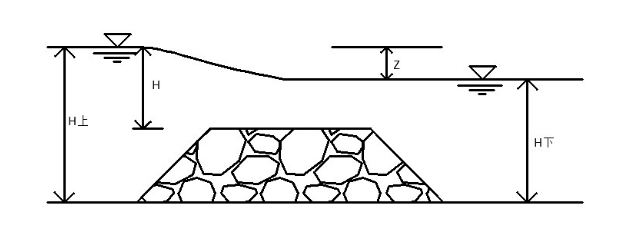
\includegraphics[width=0.6\textwidth]{yiliu.png}
    \caption{堆石体溢流示意图}
    \label{fig:dragon_port_hydraulic_calculation}
\end{figure}

水力计算主要推求内外港水位差、龙口口门处流速、口门单宽流量等水力要素随时间变化的过程线,各个水力要素指标计算公式如下所示:

内外港水位差 $Z$ 可按下式进行计算:
\begin{equation}
    Z = H_n - H_w 
\end{equation}
式中:
\begin{itemize}
    \item $Z$ —— 计算时刻内外港水位差(m);
    \item $H_n$ —— 计算时刻围区内水位(m);
    \item $H_w$ —— 计算时刻围区外水位(m)。
\end{itemize}

龙口口门处流速 $V$ 可按下式进行计算:

当 $Z < \frac{H}{3}$ 时:
\begin{equation}
    V = \varphi \sqrt{2gZ} 
\end{equation}

当 $Z \geq \frac{H}{3}$ 时:
\begin{equation}
    V = 0.54 \sqrt{2gH} 
\end{equation}

式中:
\begin{itemize}
    \item $g$ —— 重力加速度,这里取 $9.81\,\text{m/s}^2$;
    \item $\varphi$ —— 流速系数,这里取 $0.9$;
    \item $Z$ —— 上下游水位差(m);
    \item $H$ —— 堆石体顶部上游水深(m)。
\end{itemize}

龙口口门单宽流量 $q$ 可按下式进行计算:

当 $Z < \frac{H}{3}$ 时:
\begin{equation}
    q = \varphi \sqrt{2gZ(H-Z)} 
\end{equation}

当 $Z \geq \frac{H}{3}$ 时:
\begin{equation}
    q = m \sqrt{2gH^{1.5}} 
\end{equation}

式中:
\begin{itemize}
    \item $q$ —— 龙口口门单宽流量($\text{m}^3/\text{s}$);
    \item 其余参数同上。
\end{itemize}


在水量平衡方程中,龙口尺寸(龙口宽度 $B$、底槛高程 $P$)、计算时段 $\Delta t$、水力学系数($e$、$\varphi$、$m$)已经选定,计算时段终末的围区外潮位可由设计潮位过程线获得,假定围区内起始水位,通过试算法求出各个时段末围区内水位,进而获得围区内水位过程线及其他水力要素过程曲线。在这个过程中,合理准确地推求围区内水位过程线是重点和难点,具体推求步骤如下所示:

\begin{enumerate}
    \item 选择规定一个合适的计算时段 $\Delta t$,这里选取 $\Delta t = 3600\,\text{s}$;
    \item 选择龙口底槛高程或者稍微高于龙口底槛的高程作为围涂区域内起始水位;
    \item 根据已知的时刻初围区内、外水位,计算得到 $Q_{\text{溢1}}$;
    \item 假定一个水位作为计算时段末围涂区域内水位值;
    \item 根据已知的时刻末围区内、外水位,计算得到 $Q_{\text{溢2}}$;
    \item 根据时段前后流量值,计算时段前后围区库容差值;
    \item 根据围涂区域内起始水位,在围区库容曲线上对应得到计算时段初围区库容;
    \item 计算时段初围区库容和围区库容差值,求和得到计算时段末围区库容;
    \item 根据计算时段末围区库容,在围区库容曲线上对应得到计算时段末围区内水位;
    \item 如果这时得到的围区内水位与假定值一致,则认为该值为真,可以进行后续计算;否则需要重新假定时段末围涂区域内水位值再次计算上述步骤;
    \item 以上计算时段末的围区内外水位值作为下一计算时段初内外水位,重复上述步骤(1)~(10);
    \item 计算时段经过两个潮期后,若此时得到的围区内水位与步骤(2)中假定的起始水位值一致(在一定允许误差之内),则认为该值为真,计算过程结束,否则需要复查步骤(2)~(11);
    \item 以围区为横坐标,各个时段末围区内水位值为纵坐标,绘制围区内水位过程线。
\end{enumerate}


\par 
利用上述公式以及步骤,通过Python程序模拟不同龙口条件下的水力要素变化值。
%插入代码
\begin{lstlisting}[language=Python]
import math


GRAVITY = 9.81


def f(n):
    if -0.5 <= n < 1.0:
        return 775800 * n + 387900
    elif 1.0 <= n < 3.0:
        return 2118300 * n - 954600
    else:
        return 2839900 * n - 3119400

def g(m):
    if 0 <= m < 1163700:
        return (m - 387900) / 775800
    elif 1163700 <= m < 5400300:
        return (m + 954600) / 2118300
    else:
        return (m + 3119400) / 2839900


longkou_elevation = float(input("Please input the elevation of Longkou: "))
longkou_width = float(input("Please input the width of Longkou: "))
hO = float(input("Please input the initial water level: "))

# Predefined tidal levels for 24 hours (example data, adjust as needed)
A = [2.06, 3.93, 5.08, 5.40, 4.95, 3.89, 2.63, 1.49, 0.63, -0.05, -0.51, 0.02, 1.61,
     3.39, 4.89, 5.34, 4.68, 3.45, 2.22, 1.10, 0.29, -0.32, -0.73, 0.13, 2.06]

hns = hO
hws = A[0]
hnf = 4.0
s = 0.001
deltat = 3600
vs = f(hns)
velocity_max = -float('inf')
velocity_min = float('inf')

with open("Hydraulic_calculation_of_Longkou.dat", "w") as file:
    file.write(f"Elevation of Longkou: {longkou_elevation}\n")
    file.write(f"Width of Longkou: {longkou_width}\n")

    for t in range(25):
        sea_level = A[t]
        if hws < sea_level:
            jc = sea_level
        else:
            jc = hws
        
        if hws == hns:
            qls = 0
        elif hws < hns:
            if hns < longkou_elevation:
                qls = 0
            else:
                z = hns - hws
                h1 = hns - longkou_elevation
                if z >= 0.333 * h1:
                    qls = 0.385 * 0.95 * 0.9 * longkou_width * math.sqrt(2 * GRAVITY) * h1 * math.sqrt(h1)
                    velocity = -0.54 * math.sqrt(2 * GRAVITY * abs(h1))
                else:
                    qls = 0.9 * 0.95 * longkou_width * math.sqrt(2 * z * GRAVITY) * (h1 - z)
                    velocity = -1.0 * math.sqrt(2 * GRAVITY * abs(z))
                q = velocity * (h1 - z)
                velocity_max = max(velocity_max, velocity)
                velocity_min = min(velocity_min, velocity)
        else:
            if hws > hns:
                if hws < longkou_elevation:
                    qls = 0
                else:
                    h1 = hws - longkou_elevation
                    z = hws - hns
                    if z >= 0.333 * h1:
                        qls = 0.385 * 0.95 * 0.9 * longkou_width * math.sqrt(2 * GRAVITY) * h1 * math.sqrt(h1)
                        velocity = 0.54 * math.sqrt(2 * GRAVITY * abs(h1))
                    else:
                        qls = 0.9 * 0.95 * longkou_width * math.sqrt(2 * GRAVITY * z) * (h1 - z)
                        velocity = 0.9 * math.sqrt(2 * GRAVITY * abs(z)) * z / abs(z)
                    q = velocity * (h1 - z)
                    velocity_max = max(velocity_max, velocity)
                    velocity_min = min(velocity_min, velocity)
        
        vs = f(hns)
        dv = (qls) * 0.5 * deltat
        vf = vs + dv
        hf = g(vf)

        if abs(hf - hnf) < s:
            break
        else:
            hnf = hnf - 0.0001
            if hnf < 0:
                hnf = jc

   
        file.write(f"{t} {hns} {hws} {velocity} {q} {qls}\n")

    
    file.write(f"Velocity max: {velocity_max}\n")
    file.write(f"Velocity min: {velocity_min}\n")
    print(f"Velocity max: {velocity_max}")
    print(f"Velocity min: {velocity_min}")

\end{lstlisting}

利用上述程序,可以算出各个时段始末时刻的水力要素值(围区内外水位、围区内外水位差 $Z$、龙口流速 $V$、龙口单宽流量 $q$),以水力要素值为纵坐标,
以时间为横坐标,
用平滑的曲线将各点连接起来就构成了相应水力要素的过程线,
即水力要素随时间变化的规律。以龙口宽度为 200m,龙口底槛高程为 2.0m 这一情况为例。

以下表格和曲线则为该尺寸下水力要素计算成果:


\begin{table}[h!]
\centering
\caption{潮位和流量数据}
\begin{tabular}{cccccc}
\toprule
时刻 & 围区外潮位 (m) & 围区内水位 (m) & 内外水位差 (m) & 龙口流速 (m/s) & 单宽流量 (m$^3$/(s·m)) \\
\midrule
1 & 2.06 & 2.17 & 0.11 & 0.99 & 0.12 \\
2 & 3.93 & 2.82 & -1.11 & 3.02 & 4.57 \\
3 & 5.08 & 4.33 & -0.75 & 3.40 & 7.91 \\
4 & 5.40 & 5.31 & -0.09 & 1.33 & 4.40 \\
5 & 4.95 & 5.04 & 0.09 & -1.33 & -3.92 \\
6 & 3.89 & 4.14 & 0.25 & -2.21 & -4.19 \\
7 & 2.63 & 3.39 & 0.76 & -2.41 & -2.79 \\
8 & 1.49 & 2.90 & 1.41 & -2.27 & -1.46 \\
9 & 0.63 & 2.58 & 1.95 & -1.82 & -0.75 \\
10 & -0.05 & 2.41 & 2.46 & -1.53 & -0.45 \\
11 & -0.51 & 2.30 & 2.81 & -1.31 & -0.28 \\
12 & 0.02 & 2.23 & 2.21 & -1.15 & -0.19 \\
13 & 1.61 & 2.19 & 0.58 & -1.04 & -0.14 \\
14 & 3.39 & 2.57 & -0.82 & 2.82 & 2.79 \\
15 & 4.89 & 3.89 & -1 & 3.45 & 8.38 \\
16 & 5.34 & 5.26 & -0.08 & 1.25 & 4.08 \\
17 & 4.68 & 4.99 & 0.31 & -2.14 & -4.25 \\
18 & 3.45 & 3.84 & 0.39 & -2.36 & -3.42 \\
19 & 2.22 & 3.17 & 0.95 & -2.39 & -2.16 \\
20 & 1.10 & 2.75 & 1.65 & -2.07 & -1.11 \\
21 & 0.29 & 2.50 & 2.21 & -1.69 & -0.60 \\
22 & -0.32 & 2.36 & 2.68 & -1.44 & -0.37 \\
23 & -0.73 & 2.27 & 3 & -1.24 & -0.24 \\
24 & 0.13 & 2.21 & 2.08 & -1.10 & -0.16 \\
25 & 2.06 & 2.17 & 0.11 & -0.99 & -0.12 \\
\bottomrule
\end{tabular}
\end{table}


\begin{figure}[h]
    \centering
    \includegraphics[width=0.4\textwidth]{figure_1.png}
    \caption{内外港水位过程线图}
    \label{fig:hydraulic_process_line}
\end{figure}

\begin{figure}[h]
    \centering
    \includegraphics[width=0.4\textwidth]{figure_2.png}
    \caption{龙口堵口流速过程线图}
    \label{fig:hydraulic_process_line}
\end{figure}

\begin{figure}[h]
    \centering
    \includegraphics[width=0.4\textwidth]{figure_3.png}
    \caption{ 龙口堵口单宽流量过程线图}
    \label{fig:hydraulic_process_line}
\end{figure}
\newpage
通过 python 程序运算,可以研究清楚某一口门尺寸下,龙口通过设计潮型的潮流
时,各个龙口水力要素随时间的变化规律,以各个水力要素过程线进行表示。
接下来需要研究的是在龙口堵口、口门束窄的过程中,龙口口门流速及单宽流量最
大值随龙口宽度及底槛高程的变化规律。在合龙过程各个口门尺寸的情况下,从流速过
程线上分别提取在涨潮进流和落潮出流两种情况下的流速最大值,并将结果整理成表格
如下所示:

\newpage
\subsection{堵口设计}
\subsection{龙口合龙程序设计方案}

\begin{enumerate}
    \item 首先采用自卸汽车运输石方,进行平堵作业。从东、西两个石料厂运石同时进占,平堵后口门宽 200m,底槽高程 2.0m。此时最大流速 $V_{\text{max}} = 3.02\,\text{m/s}$。
    
    \item 接下来通过自卸汽车运输石方从堤两侧抛填,进行立堵作业,将龙口口门宽度缩窄为 100m,此时最大流速 $V_{\text{max}} = 3.45\,\text{m/s}$。
    
    \item 然后进行平堵作业,将龙口底槽高程抬高到 4.0m,此时龙口最大流速 $V_{\text{max}} = 2.64\,\text{m/s}$。
    
    \item 最后将口门缩至 50m,此时 $V_{\text{max}} = 2.64\,\text{m/s}$,一口气实现合龙。截流成功后紧跟着开展土方闭气工作,采用桥式土方筑堤机从围区内涂面取土,分层填筑。
\end{enumerate}
\section{环境影响评估}
白马堤工程包括隔堤和海堤以及水闸等建筑物的施工建设,施工将
影响附近海域的水文动力、泥沙冲淤变化和生态环境。环境影响分析是旨在通过
分析产生污染物的原因,提出有效的环境保护和管理的具体措施。

\subsection{水文动力影响分析}



\end{document}